%%%%%%%%%%%%%%%%%%
% Standalone document
\documentclass[notes.tex]{subfiles}
\begin{document}
%%%%%%%%%%%%%%%%%%%%%%%%%%%%%%%%%%%%%%%%%%%%%%%%%%%%%%%
%%%%%%%%%%%%%%%%%%%%%%%%%%%%%%%%%%%%%%%%%%%%%%%%%%%%%%%
\chapter{Sparticle phenomenology}
\label{chap:pheno}
%%%%%%%%%%%%%%%%%%%%%%%%%%%%%%%%%%%%%%%%%%%%%%%%%%%%%%%
%%%%%%%%%%%%%%%%%%%%%%%%%%%%%%%%%%%%%%%%%%%%%%%%%%%%%%%
In this chapter we discuss the phenomenology of supersymmetric models and how to search for low-energy particle realisations of supersymmetry in experiments. We begin by returning to supersymmetry breaking in order to define some reasonable and (partially) motivated subsets of the 124 MSSM parameters which can be used to define more constrained models. We then discuss supersymmetry at lepton and hadron colliders, and finally look at precision measurements that are indirectly sensitive to the existence of sparticles.


%%%%%%%%%%%%%%%%%%%%%%%
\section{Models for supersymmetry breaking} 
%%%%%%%%%%%%%%%%%%%%%%%
Let us begin by taking a closer look at the models we use to motivate supersymmetry breaking, and what their phenomenological consequences are. This is important to keep in mind as most searches for supersymmetry are interpreted under certain assumptions on the supersymmetry  breaking mechanism.

Generically such models can be illustrated as shown in Fig.~\ref{SSB}. There is one or more {\bf hidden sector} (HS) scalar superfield $X$ -- by hidden we mean that it has no or very small direct couplings to the MSSM fields -- that has an {\it effective (non-renormalizable) coupling} to the MSSM scalar fields $\Phi_i$ of the form
\begin{equation}
\mathcal{L}_\text{HS} = -\frac{1}{M}(\bar\theta\bar\theta)X\Phi_i\Phi_j\Phi_k,
\label{eq:HS_MSSM}
\end{equation}
where $M$ is some large scale, {\it e.g.}\ the Planck scale, that suppresses the interaction. Figure \ref{SUSYB} shows interactions that can lead to such terms, where $M$ is the mass scale of some {\bf mediator} particle $Y$. 

\begin{figure}[h!]
\centering
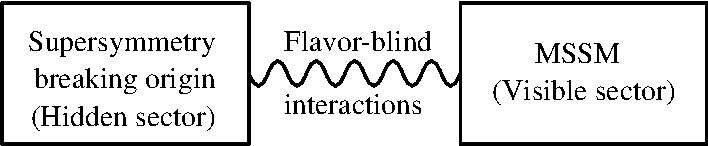
\includegraphics[scale=1.0]{figures/structure} 
\caption{A generic illustration of how to generate soft breaking terms~\cite{Martin:1997ns}. \label{SSB}}
\end{figure}

\begin{figure}[h!]
\begin{center}
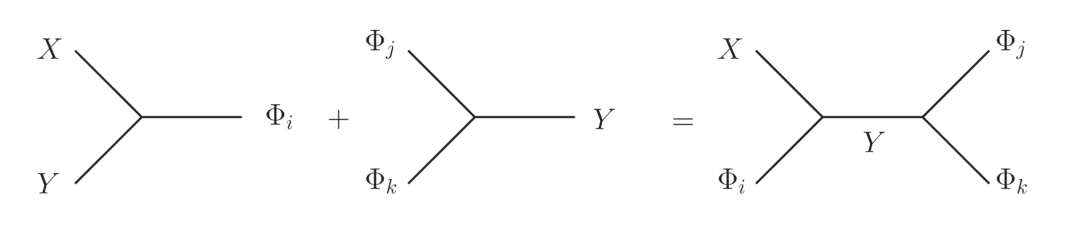
\includegraphics[scale=0.9]{figures/SUSYB} 
\caption{Interactions leading to effective 4-particle couplings in our example. \label{SUSYB}}
\end{center}
\end{figure}

If the hidden sector is constructed so that $X$ develops a vev for its auxillary $F$-component field, $F_X$,\begin{equation}
\langle X \rangle = \theta \theta \langle F_X \rangle,
\end{equation}
it breaks supersymmetry spontaneously, see the discussion leading up to Eq.~(\ref{eq:Fbreaking}). As a result, the interaction in  (\ref{eq:HS_MSSM}) will produce a soft-term of the form of the second term in Eq.~(\ref{eq:soft_terms_component_fields}),
\begin{equation}
\mathcal{L}_\text{soft}=-\frac{\langle F_X \rangle}{M}A_iA_jA_k,
\end{equation}
with the soft-mass parameter
\[m_\text{soft} = \frac{\langle F_X \rangle}{M}.\]
This has reasonable limits in that $m_\text{soft}  \to 0$ as $\langle F_X \rangle \to 0$, which is the limit of no supersymmetry breaking, and $m_{\rm soft} \to 0$ as $M \to \infty$, where the interaction with the hidden sector is decoupled because the mediating particle $Y$ becomes too heavy to have any influence. 

We will now look at two possible ways to construct such a hidden sector called Planck-scale Mediated Supersymmetry Breaking (PMSB) and Gauge Mediated Supersymmetry Breaking (GMSB).


%%%
\subsection{Planck-scale Mediated Supersymmetry Breaking (PMSB)}
%%%
In Planck-scale mediated supersymmetry breaking (PMSB) we blame some gravity mechanism for mediating the supersymmetry breaking from the hidden sector to the MSSM so that the scale of the breaking is $M = M_P = 2.4 \cdot 10^{18}$\,GeV. Then we need to have $\sqrt{\langle F_X\rangle} \sim 10^{10}-10^{11}$\,GeV in order to get $m_{\rm soft} \simeq 50-5000$\,GeV, which is roughly of the right magnitude not to re-introduce the hierarchy problem. The use of $\sqrt{\langle F_X\rangle}$ is just a conventional shorthand notation for the magnitude of the vev of whichever $F$-term that breaks supersymmetry. This is called the {\bf supersymmetry breaking scale}.

The complete soft terms for such a mechanism can then be shown to be
\begin{eqnarray}
\mathcal{L}_\text{soft} &=& -\frac{\langle F_X \rangle}{M_P}\left(\frac{1}{2} f_i \lambda^a_i \lambda^a_i + \frac{1}{6} y'_{ijk}A_i A_j A_k + \frac{1}{2}\mu'_{ij}A_iA_j + \frac{\langle F_X \rangle^*}{M_P^2}x_{ijk}A_i^*A_jA_k + {\rm c.c.}\right)\nonumber\\
 &&- \frac{|\langle F_X \rangle |^2}{M_P^2}k_{ij}A_iA_j^*.
 \end{eqnarray}
Incidentally, we can now see why we assumed the maybe-soft breaking terms to be unimportant, as  in this model they are suppressed by $|\langle F_X \rangle|/M_P^2$ compared to the other masses. 

If one assumes a minimal form for the parameters at the GUT scale, motivated by the wish for unification, {\it e.g.}\ $f_i=f$, $y'_{ijk} = \alpha y_{ijk}$, $\mu'_{ij} = \beta \mu$, and $k_{ij} = k\delta_{ij}$, then all the soft terms are fixed by just four parameters
\[m_{1/2} = f\frac{\langle F_X \rangle}{M_P}, \indent m_0^2 = k \frac{|\langle F_X \rangle|^2}{M_P^2}, \indent A_0 = \alpha \frac{\langle F_X \rangle }{M_P}, \indent B_0 = \beta\frac{\langle F_X \rangle}{M_P}.\]
The resulting phenomenology is called {\bf minimal supergravity}, or {\bf mSUGRA/CMSSM}. This is minimal in the sense of the form of the parameters, and is the most studied, but perhaps not best motivated, version of the MSSM. Usually, $B_0$ and $|\mu|$ are exchanged for $\tan\beta$ at low scales using the EWSB condition  in Eq.~(\ref{eq:EWSB_condition}), so it is common to say that there are four and a half parameters in the model: $m_{1/2}$, $m_0$, $A_0$, $\tan\beta$ and ${\rm sgn}\,\mu$.


%%%
\subsection{Gauge Mediated Supersymmetry Breaking (GMSB)} 
%%%
An alternative to PMSB is gauge-mediated supersymmetry breaking where soft terms come from {\it loop diagrams} with {\bf messenger} superfields that get their own mass by coupling to the hidden sector supersymmetry breaking  vev, and that have Standard Model gauge interactions. By dimensional analysis we must have
\[m_{\rm soft} = \frac{\alpha_i}{4\pi}\frac{\langle F \rangle}{M}.\]
If now the supersymmetry breaking scale  $\sqrt{\langle F\rangle}$ and the messenger mass $M$ are roughly comparable in size, which is reasonable given where the messenger mass comes from, then $\sqrt{\langle F \rangle} \simeq 100$\,TeV can give a viable sparticle spectrum. Notice that there is now a lot less RGE running for the parameters in the GMSB compared to the PMSB since the soft masses are created at a rather low scale.

One way of thinking about how these mass terms appear is that the messenger field(s) get masses from hidden sector vevs and contribute to for example gaugino mass terms through diagrams such as the one in Fig.~\ref{fig:GMSB}, where messenger scalars and fermions run in the loop, and their masses from the hidden sector vevs are symbolised by the mass insertions. Note that scalars can only get mass contributions like this at two-loop order since the messenger interaction is a gauge interaction, involving gauge bosons or gauginos in the MSSM. In order not to spoil GUT unification messengers are often assumed to have small mass splittings and come in $N_5$ complete $\mathbf{5} + \overline{\mathbf{5}}$ (fundamental) representations of $SU(5)$.

\begin{figure}[h!]
\begin{center}
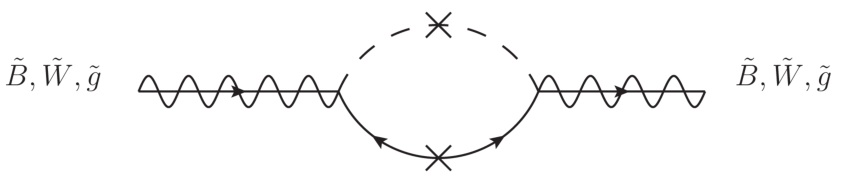
\includegraphics[scale=0.8]{figures/GMSB} 
\caption{Diagram for GMSB giving masses to the gauginos. The messenger scalars and fermions run in the loop.}
\label{fig:GMSB}
\end{center}
\end{figure}

The minimal parametrisation of GMSB models is in terms of the scale $\Lambda = \frac{\langle F\rangle}{M}$, the messenger mass $M$, the number of representations $N_5$, and $\tan\beta$ for the EWSB criterion (instead of $\mu$ and $b$). This gives the soft masses
\begin{eqnarray}
M_i &=& \frac{\alpha_i}{4\pi}\Lambda N_5,\quad\text{(gaugino masses)}\label{eq:GMSBgauginomass}\\
m_j^2 &=& 2\Lambda^2 N_5 \sum C(R)_i\left(\frac{\alpha_i}{4\pi}\right)^2,\quad\text{(scalar masses)}
\end{eqnarray}
where the sum is over the quadratic Casimir invariant for the scalar superfield $\Phi_j$ that the scalar field belongs to. We clearly see that the scalar soft-masses are a two-loop effect as discussed above. 

While this parameterisation looks independent of $M$, the messenger scale sets the starting point of the RGE running of the sparticle masses, and thus influences their magnitude. For example, the tri-linear soft-term couplings $a_{ijk}$ are expected to be very small at the messenger scale, and are effectively set to zero, however, due to RGE running they are small, but non-zero at the electroweak scale. Since the scalar masses $m_j$ scale as $\sqrt{N_5}$ compared to $N_5$ for the gauginos, we in general expect the scalars to be lighter in GMSB models. One should also notice that this parameterisation  gives the same hierarchy of gaugino masses as in mSUGRA, $M_3>M_2>M_1$, since (\ref{eq:GMSBgauginomass}) is ordered in terms of the strength of the gauge couplings $\alpha_i$. The origin of the hierarchy is different since in mSUGRA it comes from the running of the parameters down from the GUT scale.



%%%%%%%%%%%%%%%%%%%%%%
\section{Supersymmetry at lepton colliders}
%%%%%%%%%%%%%%%%%%%%%%
High-energy lepton colliders have traditionally been circular $e^+e^-$-colliders. These have the advantage of a well known centre-of-mass (CoM) energy given by the total energy of the electron--positron pair, clean final states, and periodic application of the accelerating gradient. The challenge is to reach high energies and high luminosities (collision rates). Since the electrons are light they radiate a lot of bremsstrahlung photons when bent in orbits. The highest energy so-far at an $e^+e^-$-collider was the 209 GeV CoM-energy at LEP2 in 2000. Plans are being made both for linear  $e^+e^-$-colliders, and a muon collider where there is less bremsstrahlung because of the higher muon mass, meaning that higher energies can be reached. However, there are significant technical challenges ahead for both. The linear colliders need very long installation tunnels and a very high accelerating gradient, while the muon collider must be able to produce and store the unstable muons.

Most supersymmetry searches at lepton colliders rely on the pair production of oppositely charged sparticles with electroweak couplings from $e^+e^-\to \gamma^*/Z^*\to S\bar{S}$, where $S$ symbolises a generic sparticle. Due to R-parity conservation these sparticles both decay to lighter sparticles and Standard Model decay products, until they, potentially after several successive decays known as a {\bf cascade decay}, leave only the stable LSP. This LSP must be electrically (and most likely colour) neutral due to experimental constraints on massive long-lived charged particles that would bind to atomic nuclei. The neutrality of the LSP means that it escapes detectors unseen.

The search for supersymmetry thus focuses on events with the Standard Model decay products of sparticles and an imbalance in momentum conservation due to the two missing LSPs. By the measured sum of the momenta of all the visible decay products the sum of the total momenta for the invisible particles can be inferred as going in the opposite direction. This is known as a {\bf missing energy} signature. 

In practice such missing energy measurements are challenging experimentally due to the absence of detectors near the incoming beams in the longitudinal direction, where particles that are in principle visible may escape undetected and create an artificial momentum imbalance in the longitudinal direction. At high energies this is exacerbated by the increase of collinear bremsstrahlung  from the incoming electrons at the interaction point due to interaction of the beams. This will be a particularly difficult for a future $0.5-3.0$ TeV CoM International Linear Collider (ILC) or the Compact LInear Collider (CLIC) project.\footnote{For more information on these projects see the websites for the International Linear Collider \url{http://www.linearcollider.org/} and the Compact LInear Collider \url{https://clic.cern/}}

We can now discuss more specifically the search for sfermions, neutralinos \& charginos, and Higgs bosons at lepton colliders.


%%%
\subsection{Sfermions}
%%%
We can estimate the leading order amplitude of the $s$-channel sfermion pair production process shown in Fig.~\ref{fig:LCPP}. We being by writing down the matrix element with an intermediary $\gamma$ as:
\begin{equation}
\mathcal{M} = \overline{v}ie\gamma^\mu u \frac{-ig_\mu{}_\nu}{k^2+i\epsilon}[-ie\cdot e_f (p_1-p_2)^\nu],
\end{equation}
which gives a squared matrix element of, assuming that the CoM  $s$ is much greater than $m_Z$ and taking into account both the photon and the $Z$,
\begin{equation}
|\mathcal{M}|^2 \simeq \frac{g^4 e_f^2}{8\cos\theta_W}\frac{st+(m_{\tilde{f}}^2-t)^2}{s^2}\times (1+(4\sin^2\theta_W-1)^2).
\end{equation}
Here, we take safely take $(1+(4\sin^2\theta_W-1)^2)\simeq1$. The complete differential cross-section is then:
\begin{equation}
\frac{d\sigma}{dt} = \frac{1}{32\pi}\frac{1}{s^2}|\mathcal{M}|^2.
\label{eq:sfermion_production_diff_xsec}
\end{equation}

\begin{figure}[t!]
\begin{center}
\includegraphics[width=0.5\textwidth]{figures/LCpp.eps} 
\caption{Feynman diagram for the pair production of left-handed sfermions in the s-channel at an  $e^+e^-$-collider.}
\label{fig:LCPP}
\end{center}
\end{figure}

This cross section is relatively small due to the electroweak coupling factor $g^4$ and sfermion mass suppression, so sfermion production events will be rare.
We show an example of the slepton pair production cross section including the $Z$-resonance, and the $t$-channel contributions from neutralinos (see below) in Fig.~\ref{fig:slepton_xsec}.

\begin{figure}[t!]
\begin{center}
\includegraphics[width=0.8\textwidth]{figures/sleptons.eps} 
\caption{Cross sections for selectron pair production as a function of CoM energy. Cross sections for ${\tilde e}_L^*{\tilde e}_L$ (solid line), ${\tilde e}_R^*{\tilde e}_R$ (dashed line), and ${\tilde e}_L^*{\tilde e}_R$ (dashed dotted line) are shown separately. The particular model point has a common slepton mass of $m_{\tilde e_{L/R}}=35$ GeV.}
 \label{fig:slepton_xsec}
\end{center}
\end{figure}

After production sfermions will decay, typically to a lighter neutralino or chargino and a Standard Model fermion $f$, in processes of the type $\tilde f \to f \tilde\chi_i^0$ or $\tilde f \to f' \tilde\chi_i^\pm$. Since the energy reach is limited, only the very lightest sfermions are likely to be producible, which are usually the sleptons, and these are likely to be near (but above) the mass of the lightest neutralino. See Fig.~\ref{fig:MSSMrun} for some expectations of the masses in an mSUGRA context. This means that the most expected decay is $\tilde \ell \to \ell \tilde\chi_1^0$, and  the total process is then $e^+e^-\to \tilde\ell^+\tilde\ell^- \to \ell^+\ell^- \tilde\chi^0_1\tilde\chi^0_1$, giving two oppositely charged Standard Model leptons and missing energy as the experimental signature. 

Such a (weak) signal then needs to be discriminated from Standard Model backgrounds from for example $W^+W^-$ pair production, which can lead to the final state $\ell^+\nu_\ell\ell^-\bar\nu_\ell$, featuring the same leptons and missing energy from the neutrinos. Since backgrounds are usually well under control at lepton colliders, the limit to searches is the ability to produce the sparticles at all. With a CoM energy $\sqrt{s}$ sparticles up to $\sqrt{s}/2$ are energetically possible, and a rule of thumb is that the reach approaches $\sqrt{s}/2$ from below given sufficient data, never quite  getting to $\sqrt{s}/2$.

Should some excess be discovered, we need a smoking duck in order to confirm that this is indeed supersymmetry.  We would like to identify and measure the masses of as many new particles as possible, and hopefully also their spin. The properties of the sparticles can be measured through the inferred cross section, and the kinematical distribution of the final state products. The ability of a lepton collider to easily change the CoM energy $\sqrt{s}$, allows for a so-called {\bf threshold scan} of the cross section where the cross section is measured as a function of $\sqrt{s}$ around where it becomes zero. This in turn allows for a very precise measurement of the mass of the pair produced particle. As an example of a kinematic distribution, for the process discussed here, it can be shown that the energy distribution for the final state leptons is a uniform distribution between $E_{\rm min}$ and $E_{\rm max}$ where
\begin{equation}
E_{\rm max/min} =\frac{\sqrt{s}}{4}\left(1-\frac{m^2_{\tilde{\chi}^0_1}}{m_{\tilde{l}}^2}\right)\left(1\pm \left(1-\frac{4m_{\tilde{l}}^2}{s}\right)^{1/2}\right),
\end{equation}
which, with a known slepton mass, also gives a handle on the LSP mass $m_{\tilde\chi^0_1}$ even though it is undetected.


%%%
\subsection{Neutralinos \& charginos}
%%%
For charginos and neutralinos the production cross section depends on their wino, bino and higgsino components. You would be forgiven to think that pair production of the lightest neutralino $e^+e^- \to \tilde{\chi}^0_1\tilde{\chi}^0_1$ would be the natural sparticle to search for, however, this has some significant problems. Since it is usually the LSP it does not decay, and there is nothing in the event that can actually be measured. We cannot use the missing energy as that requires an {\it imbalance} in momentum. Given sufficiently hard (energetic) radiation from either the initial electron or positron, a single photon recoiling against missing energy could potentially be measured, and this, so-called {\bf mono-photon search}, was indeed a search channel for dark matter production at LEP. However, for neutralino dark matter this does not work all that well for other reasons. The $Z\tilde\chi_i^0\tilde\chi_j^0$ vertex shown in Fig.~\ref{fig:ZNN}  has the Feynman rule 
\begin{equation}
\frac{ig}{2\cos\theta_W}\gamma^\mu\left[\left(N_{i3}N^*_{j3}-N_{i4}N^*_{j4}\right)P_L-\left(N^*_{i3}N_{j3}-N^*_{i4}N_{j4}\right)P_R\right],
\label{eq:ZNN_vertex}
\end{equation}
which depends only on the higgsino components of the neutralinos, $N_{i3}$ and $N_{i4}$. This can be understood from the fact that there are no $ZZZ$ or $Z\gamma\gamma$ vertices in the Standard Model that can be supersymmetrised, only a $Zhh$ vertex. For the photon there is no tree level coupling to the neutralinos at all since there are no direct couplings between the Higgs and the photon in the Standard Model. Thus, only neutralinos with significant higgsino components can be produced this way. To top it off, a light higgsino with a mass dominated by the $\mu$ parameter would have very similar values of $N_{i3}$ and $N_{i4}$, thus canceling the coupling.

\begin{figure}[h!]
\begin{center}
\includegraphics{figures/Zgaugino.eps} 
\caption{Vertex for $Z\tilde\chi_i^0\tilde\chi_j^0$.}
\label{fig:ZNN}
\end{center}
\end{figure}

The selectron and electron sneutrino have a special r\^ole for $e^+e^-$ colliders due to the resulting $t$-channel diagrams. Figure \ref{fig:tdiag} shows the $t$-channel diagrams that are important in pair production at a $e^+e^-$ collider.  
Neutralino pair production with $t$-channel selectron exchange does not suffer from the same problems as neutralino pair production in the $s$-channel. However, the process depends on the selectron mass as $m_{\tilde e}^{-4}$ for large mass values and is rapidly suppressed.

\begin{figure}[h!]
\begin{center}
\includegraphics[width=\textwidth]{figures/tdiaglc.eps} 
\caption{The $t$-channel diagrams for pair production of a) selectrons and electron sneutrinos, and b) neutralinos and charginos.}
\label{fig:tdiag}
\end{center}
\end{figure}

The consequences of the above discussion is that it is the production of the second lightest neutralino and the lightest chargino that is typically searched for in the combinations $\tilde\chi_2^0\tilde\chi_1^0$, $\tilde\chi_2^0\tilde\chi_2^0$, and $\tilde\chi_1^+\tilde\chi_1^-$. These decay -- unless there is a slepton with a mass intermediary to the produced particle and the LSP -- to the LSP and a possibly off-shell vector boson, $\tilde\chi_2^0\to Z^{(*)}\tilde\chi_1^0$ and $\tilde\chi_1^\pm\to W^{(*)}\tilde\chi_1^0$. Thus the expected  experimental signature is the fermionic decay products of the vector bosons with additional missing energy from the LSPs. 

If the mass relevant differences between the neutralinos and charginos are small then the resulting decay products of the off-shell vector bosons will have little energy -- the technical term for this is that they are {\bf soft}, as opposed to very energetic particles that are {\bf hard}. Soft particles are difficult to reconstruct in detectors, and events dominated by soft particle production are easily missed, meaning that degenerate scenarios are difficult to discover, and sparticles mass bounds become very poor in this case. This is particularly unfortunate since a scenario where $\mu\ll M_1,M_2$ is well motivated on theoretical grounds, and with $\mu$ controlling two neutralino masses and one chargino, the lightest two neutralinos and the lightest chargino indeed become degenerate.


%%%
\subsection{Higgs bosons}
%%%
Because of the very small Yukawa coupling of electrons, Higgs bosons are not expected to have significant direct production cross sections at a $e^+e^-$ collider. The most realistic production channels are Higgs-strahlung where the Higgs boson is attached to a vector boson: $e^+e^-\to Zh$, $e^+e^-\to ZH$, $e^+e^-\to Ah$ and $e^+e^-\to AH$, charged Higgs pair production $e^+e^-\to H^+H-$, and $W^+W^-$ vector boson fusion into Higgs bosons $e^+e^-\to \nu_e\bar\nu_e h(H)$. 


%%%
\subsection{Current bounds at lepton colliders}
%%%
The below bounds are all from the LEP (Large Electron Positron) collider, running from 1989 until 2000, which outdated all previous bounds with a top energy of $\sqrt{s}=209$ GeV, recording an integrated luminosity (amount of data) of 233~pb$^{-1}$ above 204 GeV. Results exist from all four LEP experiments ALEPH, DELPHI, L3 and OPAL.\footnote{Most of which are silly acronyms of course.} The numbers below are all taken from the 2014 PDG (Particle Data Group) review~\cite{Agashe:2014kda}, but the conclusions from the LEP data has changed little since then. 

While these bounds often come from pair-production of the relevant sparticles, and thus are less model dependent than the hadron collider bounds presented in the next section, there remains some model dependence in many results, which, unfortunately, is sometimes ignored in the literature. Complicating matters is a reliance by the LEP experiments on theoretical assumptions such as GUT-scale coupling and gaugino mass unification in many searches.
\begin{itemize}
\item Selectron: The strongest limit given is $m_{\tilde{e}_L}>107$ GeV and $m_{\tilde{e}_R}>73$ GeV (ALEPH 2002) in searches for acoplanar di-electrons.\footnote{The observant reader will notice that two electrons are always in the same plane, however, when experimentalists say acoplanar, they mean not in one plane with the beam axis.} However, the limit is the result of a scan over MSSM parameter space simplified by assuming a common $m_0$ and $m_{1/2}$ at GUT scale. Interpreted in the even more constrained mSUGRA with $A_0=0$ the bounds are even stronger, 152 GeV and 95 GeV, respectively. In contrast, due to strict limits on the precisely measured $Z$-width, there is a fully model independent limit of $m_{\tilde{e}_{L/R}}>40$ GeV.\footnote{Similar model independent limits around half the $Z$-mass exists for all sparticles that couple to the $Z$.}
\item Smuon: $m_{\tilde{\mu}_R}>94$ GeV (DELPHI 2003). The limit is obtained as in the MSSM scenario for the selectron.
\item Stau: $m_{\tilde{\tau}_1}>81.9$ GeV (DELPHI 2003) assuming exclusive $\tilde{\tau}_1 \to \tau \tilde{\chi}^0_1$ decays and $m_{\tilde{\tau}_1} - m_{\tilde{\chi}^0_1}> 15$ GeV.
\item Sneutrinos: From  LEP we have an indirect limit of  $m_{\tilde{\nu}}>94$ GeV (DELPHI 2003) in neutralino \& slepton searches. This assumes $m_{\tilde{e}_R} - m_{\tilde{\chi}^0_1}>10$ GeV. From the Z-width we can obtain the model independent limit $m_{\tilde{\nu}}> 44.7$ GeV. 
\item Neutralino: The limit $m_{\tilde{\chi}^0_1}> 46$ GeV (DELPHI 2003) has been derived from the direct searches for $\tilde{\chi}^0_1 \tilde{\chi}^0_2$ and $\tilde{\chi}^0_2 \tilde{\chi}^0_2$. This assumes gauge coupling unification and a common gaugino mass $m_{1/2}$ at GUT scale. Even in the $Z$-decays, the contribution to the width depends on the higgsino component of the lightest neutralino, so $m_{\tilde{\chi}^0_1} \simeq 0$ GeV is still in principle allowed~\cite{Dreiner:2009ic}.
\item Here we have $m_{\tilde{\chi}^\pm_1}\geq 94$ GeV (DELPHI 2003), assuming GUT scale universality of $m_0$ and $m_{1/2}$ and using multiple direct search channels from production of charginos, neutralinos and sleptons. It also assumes either no third generation sfermion mixing or $m_{\tilde{\chi}^\pm_1} - m_{\tilde{\chi}^0_1}>6$ GeV. From the $Z$-width we can extract a strict limit of $m_{\tilde{\chi}^\pm_1}\geq 45$ GeV.
\end{itemize}




%%%%%%%%%%%%%%%%%%%%%%
\section{Supersymmetry at hadron colliders}
%%%%%%%%%%%%%%%%%%%%%%
Since the particles collided at hadron colliders (protons and other nuclei) are heavier they are not as susceptible to loosing energy through bremsstrahlung as the light leptons. Thus they can more readily be accelerated in a circular collider with periodic acceleration. However, this mass both means that linear colliders are inappropriate since the acceleration is smaller for the same applied fields, and that it is more difficult to steer the hadrons in a circular orbit. Thus the energy available at a hadron collider is limited by the strength of the bending magnets.

Up to 2009 the highest energy hadron collider was the Tevatron based at Fermilab outside of Chicago, that collided protons and anti-protons at $\sqrt{s}=1.96$ TeV. The current record is held by the Large Hadron Collider (LHC) at CERN, colliding protons at a top energy of $\sqrt{s}=13$ TeV.\footnote{The LHC was designed to operate at $\sqrt{s}=14$ TeV, but has had problems fully reaching that energy. In the next round of the LHC to start in 2022, called Run III, the plan is to go to $\sqrt{s}=13.5$ TeV.}

Since a proton--proton collider mostly collides partons, the quarks and gluons inside the protons, and since the strong coupling is large, this means that we can get large cross sections and potentially many events for QCD charged sparticles, {\it i.e.}\ squarks and gluinos, provided their masses are low enough. Cross sections for particles that have only electroweak charges (sleptons, electroweakinos, Higgs bosons) are expected to be considerably smaller, however, these sparticles are also expected to be lighter. The balance between these factors means that both types of sparticles are searched for.

As discussed earlier, with R-parity conservation sparticles are produced in pairs and both decay to the LSP. In Fig.~\ref{fig:SPS1a_spectrum} we show the sparticle mass spectrum for a particular mSUGRA benchmark point called SPS1a that has $m_0=100$ GeV, $m_{1/2}=250$ GeV, $A_0=-100$ GeV, $\tan\beta=10$ and $\text{sgn}\,\mu=+$~\cite{Allanach:2002nj}.\footnote{This benchmark point is now quite old and clearly excluded by searches, but it still serves as a nice illustration of the kind of sparticle spectrum expected in mSUGRA models.}
By producing the squarks or gluinos near the top of the mass spectrum in a collision we see that we can get many different quite long decay chains, called cascades. We illustrate such an event in  Fig.~\ref{fig:cascade}.

\begin{figure}[t!]
\centering
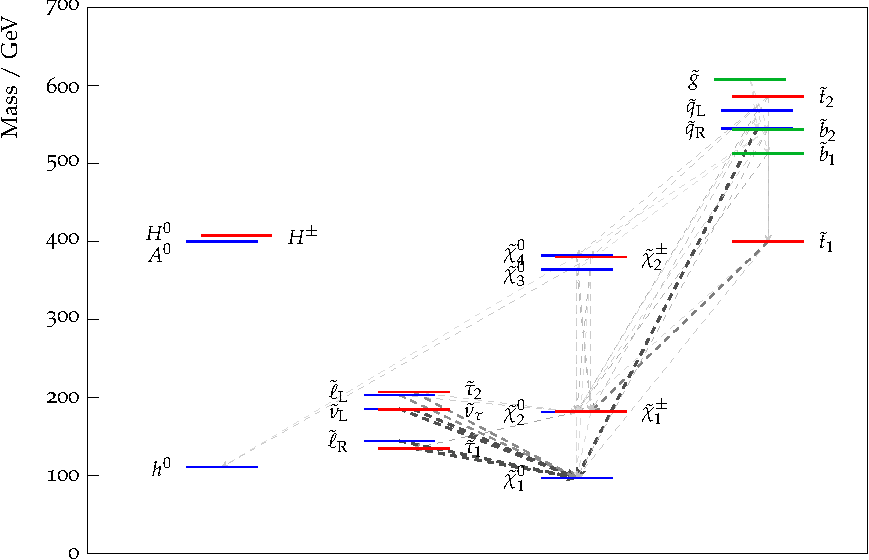
\includegraphics[width=0.9\textwidth]{figures/sps1a} 
\caption[Cascades for SPS1a]{Supersymmetric particle mass spectrum (coloured solid lines)  and possible decay channels (dashed lines) for the SPS1a benchmark point. Only decays with branching rations above 5\% are shown. The line opacity indicates relative branching ratios. This plot was generated using {\tt PySLHA~3.0.1}~\cite{Buckley:2013jua}. }
\label{fig:SPS1a_spectrum}
\end{figure}

%%%
\begin{figure}[h]
\centering
\begin{tikzpicture}
\begin{feynman}
%
\diagram [layered layout, horizontal=B to C] {
B [blob]  -- [fermion, edge label=$\tilde g$] C  -- [scalar, edge label=$\tilde q$] D  -- [fermion, edge label=$\tilde\chi_2^0$] E -- [scalar, edge label=$\tilde e_L^*$] F -- [fermion] G [particle=$\tilde\chi_1^0$],
C -- [anti fermion] c [particle=$\bar q$],
D -- [fermion] d [particle=$q$],
E -- [fermion] e [particle=$e^-$],
F -- [anti fermion] f [particle=$e^+$],
B --  [scalar, edge label=$\tilde q$] C2  -- [fermion, edge label=$\tilde\chi_2^0$] D2  -- [fermion, edge label=$\tilde\chi_1^0$] E2,
C2 -- [fermion] c2 [particle=$q$],
D2 -- [boson, edge label=$Z$] d2 -- [fermion] d3 [particle=$\mu^-$],
d2-- [anti fermion] d4 [particle=$\mu^+$],
A1 [particle=$q$] -- [fermion] B,
A2 [particle=$g$] -- [gluon] B,
};
\end{feynman}
\end{tikzpicture}
\caption{Cascade decays starting with the production of a gluino and squark pair from a gluon--quark interaction.}  
\label{fig:cascade}
\end{figure}
%%%

In hadron collisions the momenta of the incoming partons is unknown, so no complete momentum balance can be made. However, the sum of the momenta in the direction transverse to the beam direction is zero. Thus with escaping LSPs we can observe  {\bf missing transverse energy}, $\slashed{E}_T$ or $E_T^\text{miss}$, {\it i.e.}\ an imbalance in the directional sum of all energy deposits transverse to the beam direction. The rest of the signal depends on which sparticles are searched for. In broad terms this means that if searching for gluino of squark production then at some point the cascade decay must shed colour charge to arrive at the LSP, resulting in Standard Model quarks or gluons that hadronise and produce jets in the detector (hadronic showers). If instead searching for electroweakly produced sparticles or Higgs bosons, one usually assumes an absence of significant jet activity, and instead looks for leptons from the decays of the sleptons or electroweakinos, possibly through vector bosons.

At the LHC the Standard Model backgrounds are much more significant and problematic. For example, at design luminosity the LHC produces about 10 pairs of top quarks per second. Due to the top quark decay $t\to bW^+$, resulting in charged leptons and potential missing energy from neutrinos in $W$ decays, as well as jets produced in hadronic $W$ decays and from the $b$-quarks, this alone is a significant background to many supersymmetry searches. Figure~\ref{fig:LHCbackground} shows the expected backgrounds and signals produced in different channels at the $\sqrt{s}=14$ TeV LHC for different assumed particle masses. One can see that even the largest supersymmetric cross sections that we get for squark and gluino production are orders of magnitude below the Standard Model backgrounds for masses beyond 500 GeV.

\begin{figure}[h!]
\centering
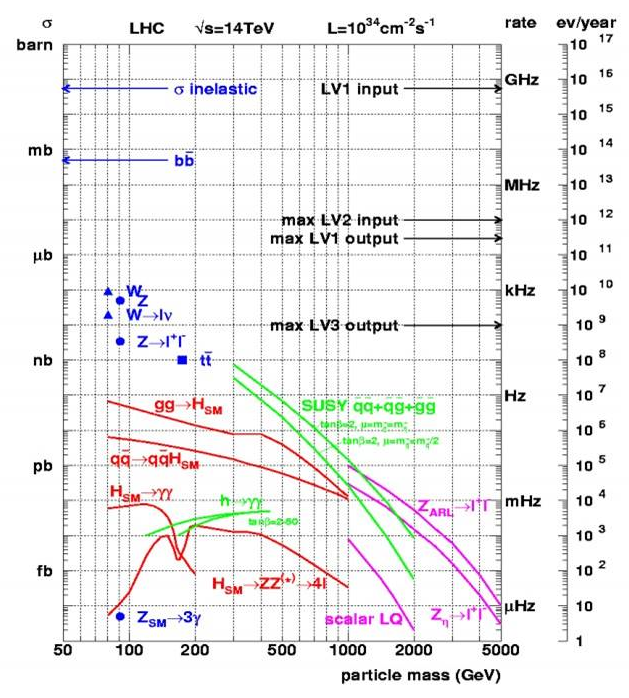
\includegraphics[width=0.7\textwidth]{figures/background} 
\caption{Plot of the expected cross sections and rates for various processes at the $\sqrt{s}=14$~TeV LHC plotted against the mass of the particles, assuming the design final luminosity of the LHC (rate of data taking). The current Run II of the LHC has collected around 140~fb$^{-1}$ of data, so the lowest point on the cross section axis indicates that $\mathcal{O}(1)$ events are expected to have been produced by now.}
\label{fig:LHCbackground}
\end{figure}

To cope with this challenge, the searches define kinematical variables that are designed to separate supersymmetry events from Standard Model events. For example, searching for the production of squarks and/or gluinos decaying to the LSP, one expects jets and missing energy from two LSPs. One can then define the {\bf effective mass}
\begin{equation}
M_{\rm eff} = \sum p_T^{\text{jet}} + \slashed{E}_T,
\label{eq:Meff}
\end{equation}
from the sum of the transverse momentum of the jets in the event, $p_T$, and the missing energy. The expectation is then that this is more significant in squark and gluino production events than in Standard Model events, so that a high requirement on $M_{\rm eff}$ reduces the number of background events without significantly removing events with sparticles. This helps for example to combat $t\bar t$ production because the jet $p_T$s in those events are limited by the energy in the top quark mass, while the more massive squarks and gluinos will have higher jet $p_T$s.

However, there are also models where this kind of approach is ineffective. Imagine a scenario where only the lightest stop $\tilde{t}_1$ is light enough to be copiously produced. If $m_{\tilde{t}_1} - m_{\tilde{\chi}^0_1}< m_W$ then the stop will dominantly decay as $\tilde{t}_1 \to c\tilde{\chi}^0_1$ or $\tilde{t}_1 \to b l \nu \tilde{\chi}^0_1$, where all final state particles have rather low energy ($p_T$), so-called {\bf soft particles}. 
As for the degenerate neutralino scenario discussed above, this is very difficult to discover with standard techniques.

%One alternative to jets and lots of missing energy is to look for leptons (and some small missing energy) from gaugino pair production and decays. Searching the lepton and missing energy channels is a very effective way to isolate any production of sparticles from SM backgrounds, but for setting bounds it is bad since the only model independent production is {\bf Drell-Yan} production, {\it e.g.}\ $q\overline{q}\to (Z/\gamma)^*\to\tilde{\chi}^0_1\tilde{\chi}^0_2,\tilde{\chi}^{+}_1\tilde{\chi}^{-}_1,\tilde{l}_L^*\tilde{l}_L,\tilde{l}_R^*\tilde{l}_R$, and $q'\overline{q}\to W^*\to\tilde{\chi}^0_2\tilde{\chi}^\pm_1$, which all have low cross sections due to the smaller electroweak coupling and the smaller anti-quark content of the proton. The expected bounds from such searches for the mSUGRA model is compared to other searches in Fig.~\ref{fig:reach}.
%
%\begin{figure}[h!]
%\centering
%\includegraphics[scale=0.5]{figures/reach.eps} 
%\caption{Plot of the projected discovery reach for different values of $m_{1/2}$ and $m_0$ in the mSUGRA model with 100~fb$^{-1}$ or 300~fb$^{-1}$ of data at the Compact Muon Spectrometer (CMS). The light blue area represents theoretical restrictions on the parameter space. The dark blue area is the parameter space that was probed by the Tevatron. The red lines represents a pure jets pluss $\not\! E_T$ search at 14\,TeV. The blue lines represent searches using leptons. The dotted lines show the masses of different sparticles in this parameter space. \label{fig:reach}}
%\end{figure}

Another example of the use of kinematics is the distribution of invariant masses. In  Fig.~\ref{fig:gen_cascade} we show an example of two sequential  two-body decays. Even if particle $A$ here is invisible, for example the LSP, we can use two visible decay products $a$ and $b$ to form the invariant mass $m_{ab}$. One can show that the distribution for $m_{ab}$ has a triangular shape with a sharp endpoint at the maximum
\begin{equation}
(m_{ab}^{\max})^{2} = \frac{\left(m_{C}^{2}-m_{B}^{2}\right)
\left(m_{B}^{2}-m_{A}^{2}\right)}{m_{B}^{2}}, 
\label{eq:m_ab}
\end{equation}
where we have assumed that $a$ and $b$ are massless.\footnote{A more complicated expression covers the massive case.}  This can be used both to select events that potentially have supersymmetric particles in them depending on the value of the invariant mass, and to determine relationships between the sparticle masses. In Fig.~\ref{fig:mab_measurement} we show a simulation of the invariant mass distribution of two opposite-sign same-flavour  (OSSF) leptons $m_{\ell\ell}$ from the production of $\tilde\chi_2^0$ and its decay chain $\tilde\chi_2^0\to \ell^\pm\tilde\ell_R^\mp \to \ell^\pm\ell^\mp\tilde\chi_1^0$. 

%%%
\begin{figure}[h]
\centering
\begin{tikzpicture}
\begin{feynman}
%
\diagram [layered layout, horizontal=B to A] {
C -- [edge label=$C$] B  -- [edge label=$B$] A  -- [edge label=$A$] E,
B -- b [particle=$b$],
A -- a [particle=$a$],
};
\end{feynman}
\end{tikzpicture}
\caption{A generic illustration of two successive two-body decays $C\to bB$ and $B\to aA$.}  
\label{fig:gen_cascade}
\end{figure}
%%%

%%%
\begin{figure}[h!]
\centering
\includegraphics[width=0.8\textwidth]{figures/p250_OSOF_mll.eps} 
\caption{Invariant mass distribution of opposite sign same flavour (OSSF) dileptons for the mSUGRA benchmark model point SPS1a~\cite{Gjelsten:2004ki}.}
\label{fig:mab_measurement}
\end{figure}
%%%

As alternatives to these standard searches for pair produced sparticles with missing energy there are ongoing searches for decaying LSPs when R-parity is violated, or the production of single sparticles.\footnote{Single sparticle production at the LHC requires rather large R-parity violating couplings for the $LQ\bar D$ or $\bar U \bar D\bar D$ operators, of the order of $\lambda > 10^{-2}$.} There is also the possibility of {\bf massive metastable charged particles} (MMCPs), typically in scenarios with a gravitino LSP, where the next-to-lightest supersymmetric particle (NLSP) is charged and long-lived because the decay to the gravitino is via a very weak gravitational coupling. The latter also includes so-called {\bf R-hadrons} if the NLSP has colour charge, which means that it will hadronise after production and be a short-lived but very massive meson or baryon. We should also mention the searches for the extra Higgs states predicted in the MSSM.\footnote{But we don't really have time.}


%%%%%%%%%%%%%%%%%%%%%%%
\section{Current bounds on sparticle masses}
\label{sec:current_LHC_bounds}
%%%%%%%%%%%%%%%%%%%%%%%
The LHC has finished its Run II and collected a total of around 140 fb$^{-1}$ of data per experiment at $\sqrt{s}=13$ TeV of energy. It is currently preparing for Run III to start in 2022.  Direct bounds from the LHC experiments ATLAS and CMS now supersede bounds from other colliders (Tevatron and LEP) in almost all channels, with some exceptions for models with degenerate masses. The below limits are mostly limits with the full Run II dataset and represent the current state-of-art in sparticle searches. We mostly use examples from ATLAS, the corresponding plots from CMS are very similar.

The strongest current limits in terms of mass are on the gluino and squarks simply because of the large production cross sections. Significant bounds on electroweakinos and sleptons exist, but these are either model dependent (depend on squark/gluino mass assumptions and cascade decays), or weaker if the rely only on electroweak production.

%%%
\subsection{Squarks and gluinos}
In Fig.~\ref{fig:msugra_squarkgluinolimit} we show the limits from the ATLAS experiment on the mSUGRA model using searches for jets plus missing energy with all the data collected at 8 TeV. The mSUGRA parameters $\tan\beta$ and $A_0$ have been chosen in order to give relatively large Higgs masses for small values of $m_{1/2}$ and $m_0$. The figure also shows the corresponding first and second generation squark masses, the gluino mass (both dot-dashed lines), and the Higgs mass (purple) for these parameter values. We then have the following approximate bounds in mSUGRA: $m_{\tilde{q}}>1600$\,GeV and $m_{\tilde{g}}> 1100$\,GeV. Bounds on the mSUGRA space directly have not been updated since this plot.

%%%
\begin{figure}[t!]
\begin{center}
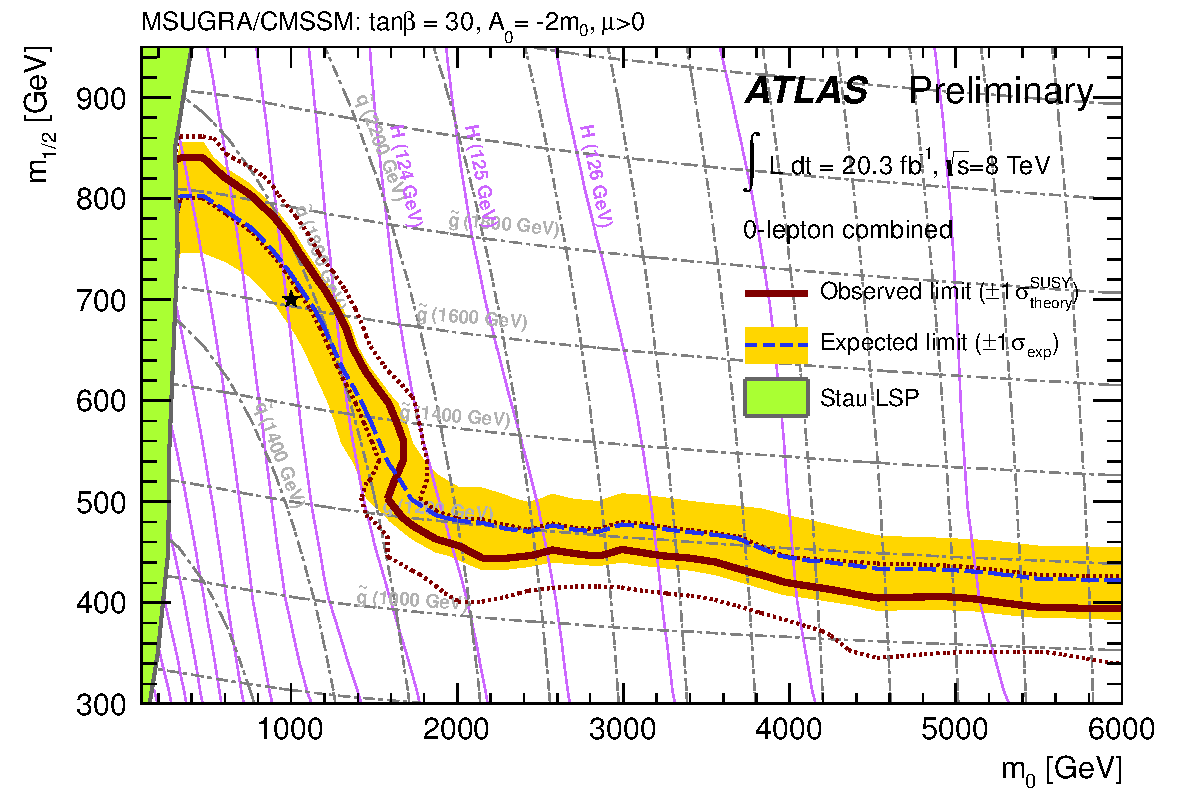
\includegraphics[width=0.9\textwidth]{figures/mSUGRA_0lep_limit} 
\caption{Plot of the excluded area in the $m_{1/2}$-$m_0$ plane of the mSUGRA parameter space for $\tan\beta=30$, $A_0=-2m_0$ and $\mu >0$ for searches using missing energy and jets. The limit is the red line. The green area is theoretically forbidden because it has a charged LSP (the stau)~\cite{ATLAS-CONF-2013-047}.}
\label{fig:msugra_squarkgluinolimit}
\end{center}
\end{figure}
%%%

Notice that in the figure the squark mass bound is more or less equivalent to the mass required for a sufficiently heavy Higgs, thus the direct search does not constrain the squarks masses significantly more here than the indirect constraint from the Higgs mass. 

An important question is how these bounds change as we move away from the mSUGRA assumptions. In mSUGRA the resulting gluino and squark decays are very much constrained by the model. For more general models the limits depend on what decay chains are dominant. In Fig.~\ref{fig:gluino_squarklimit} we show current limits in the gluino--lightest neutralino and squark--lightest neutralino mass planes under various assumptions on the decay chain shown in different colours. 

%%%
\begin{figure}[t!]
\begin{center}
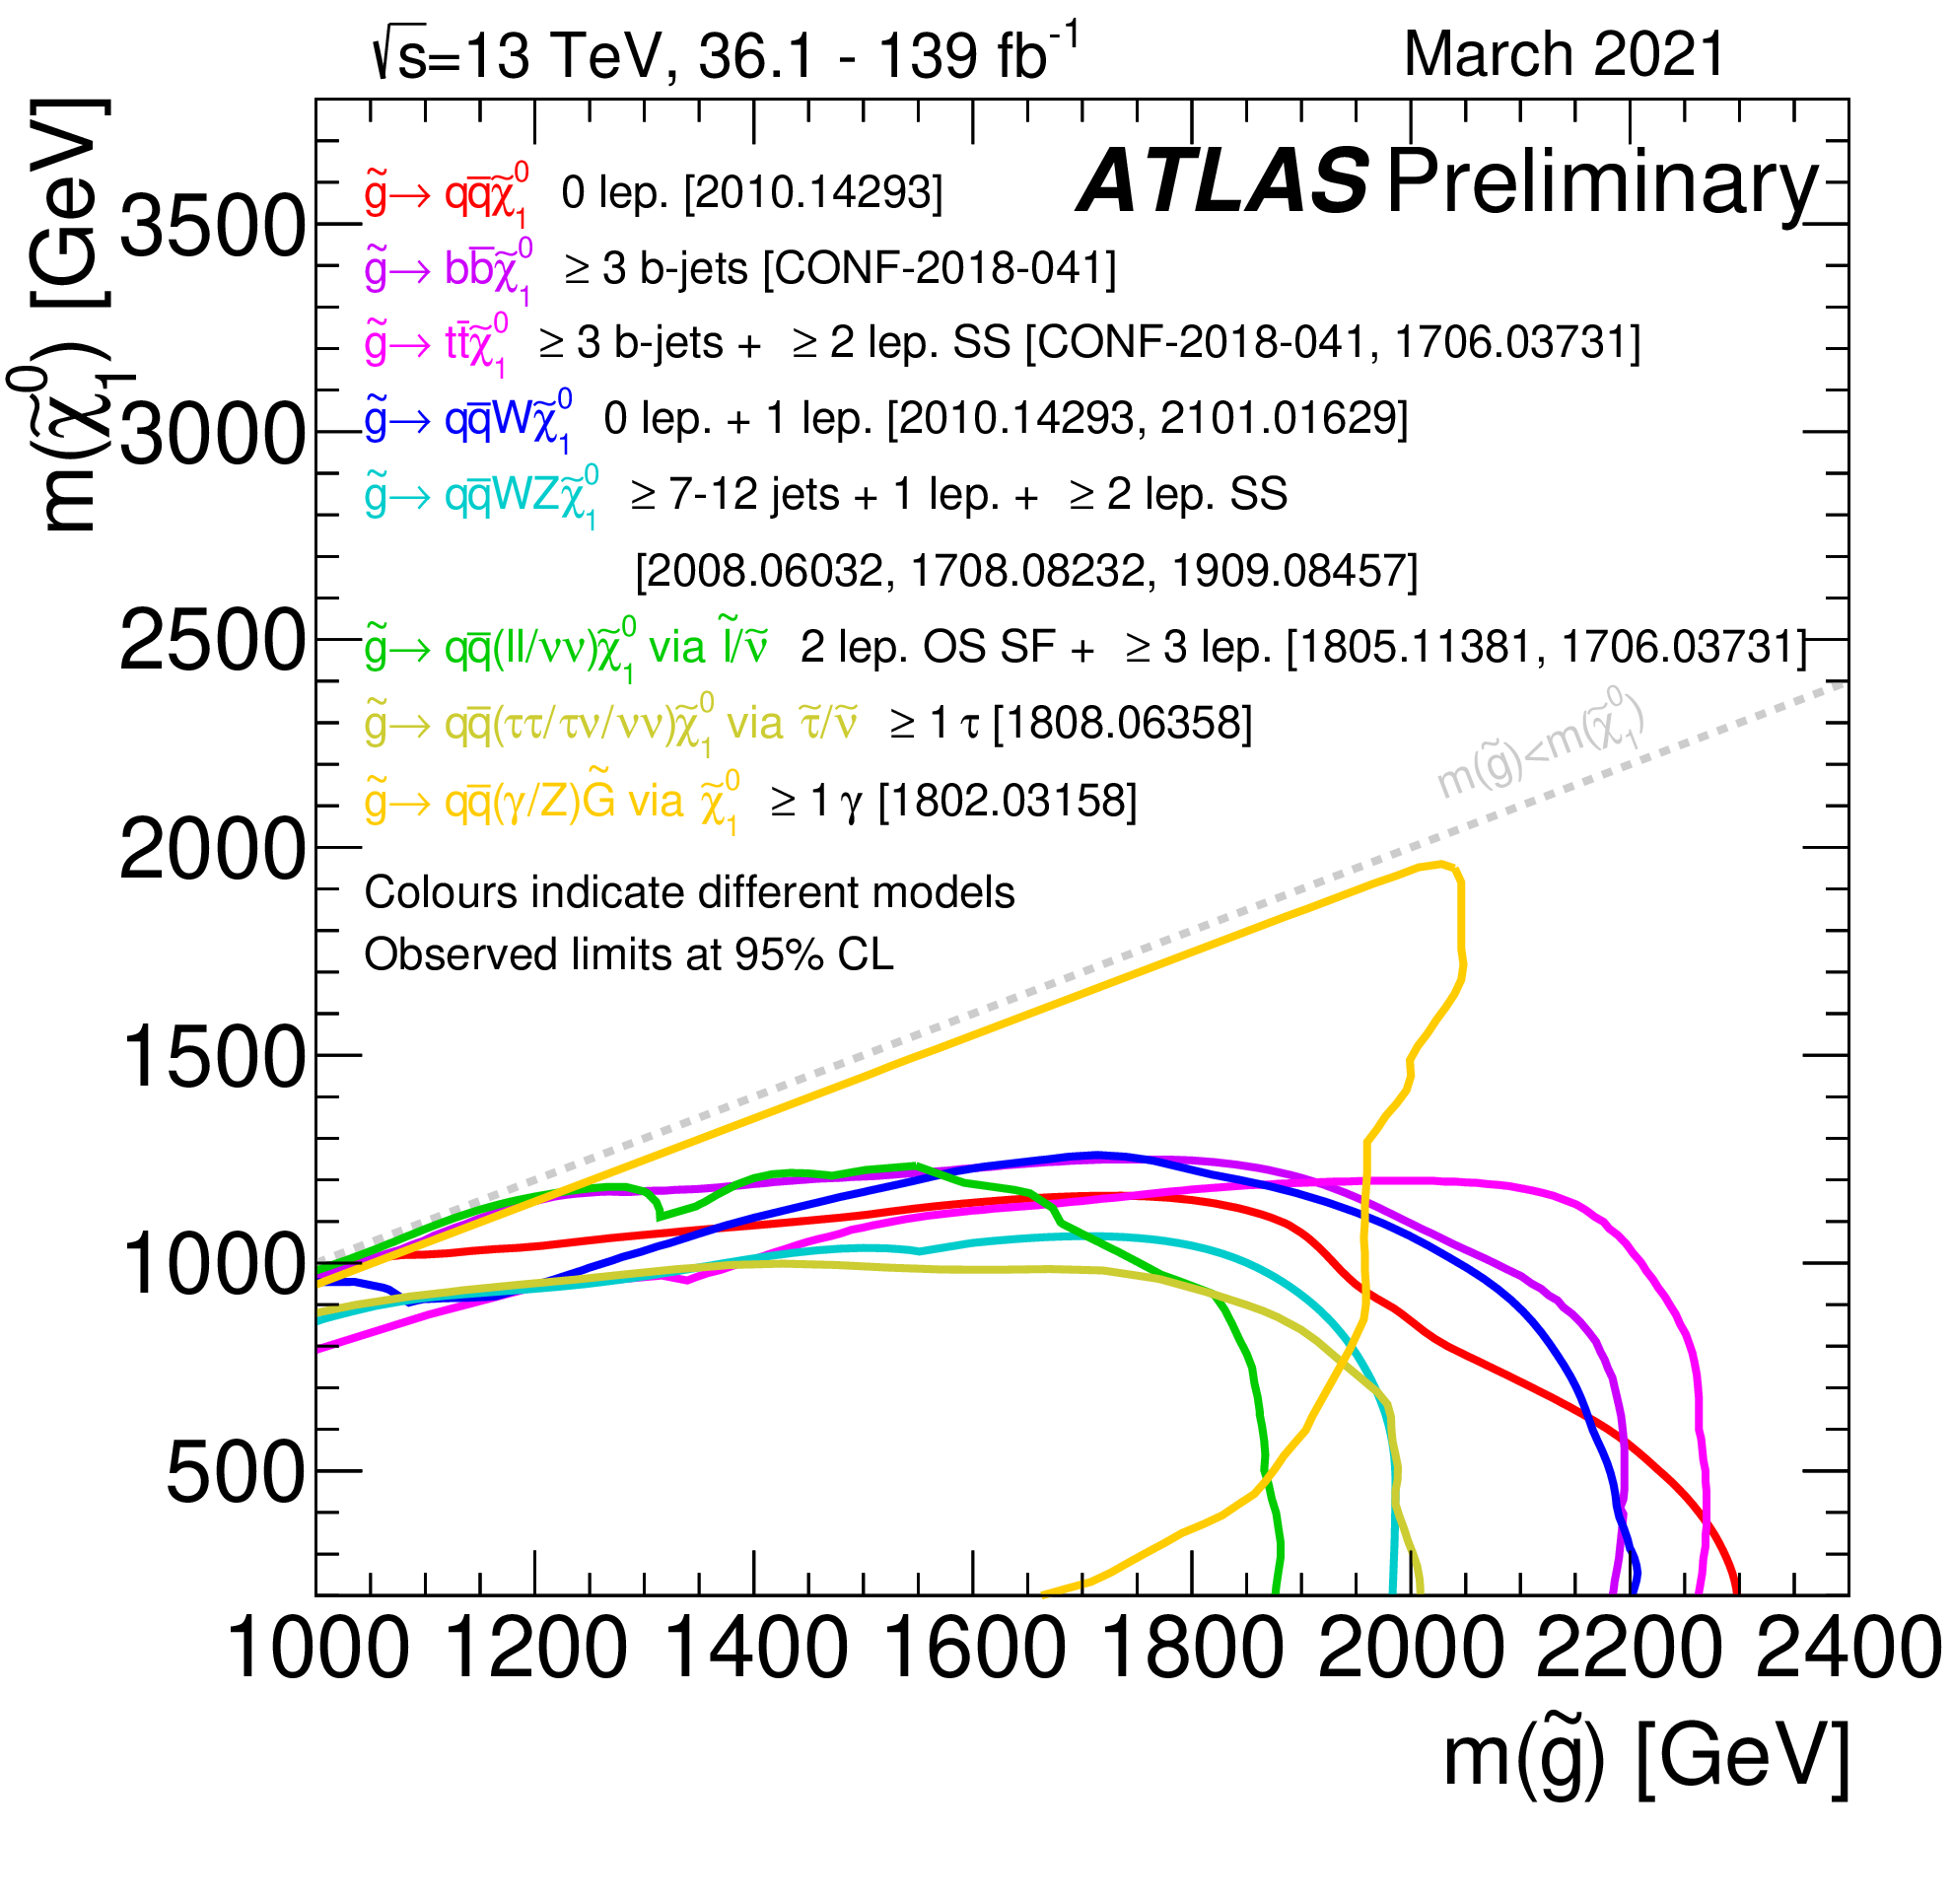
\includegraphics[width=0.49\textwidth]{figures/gluino_limit} 
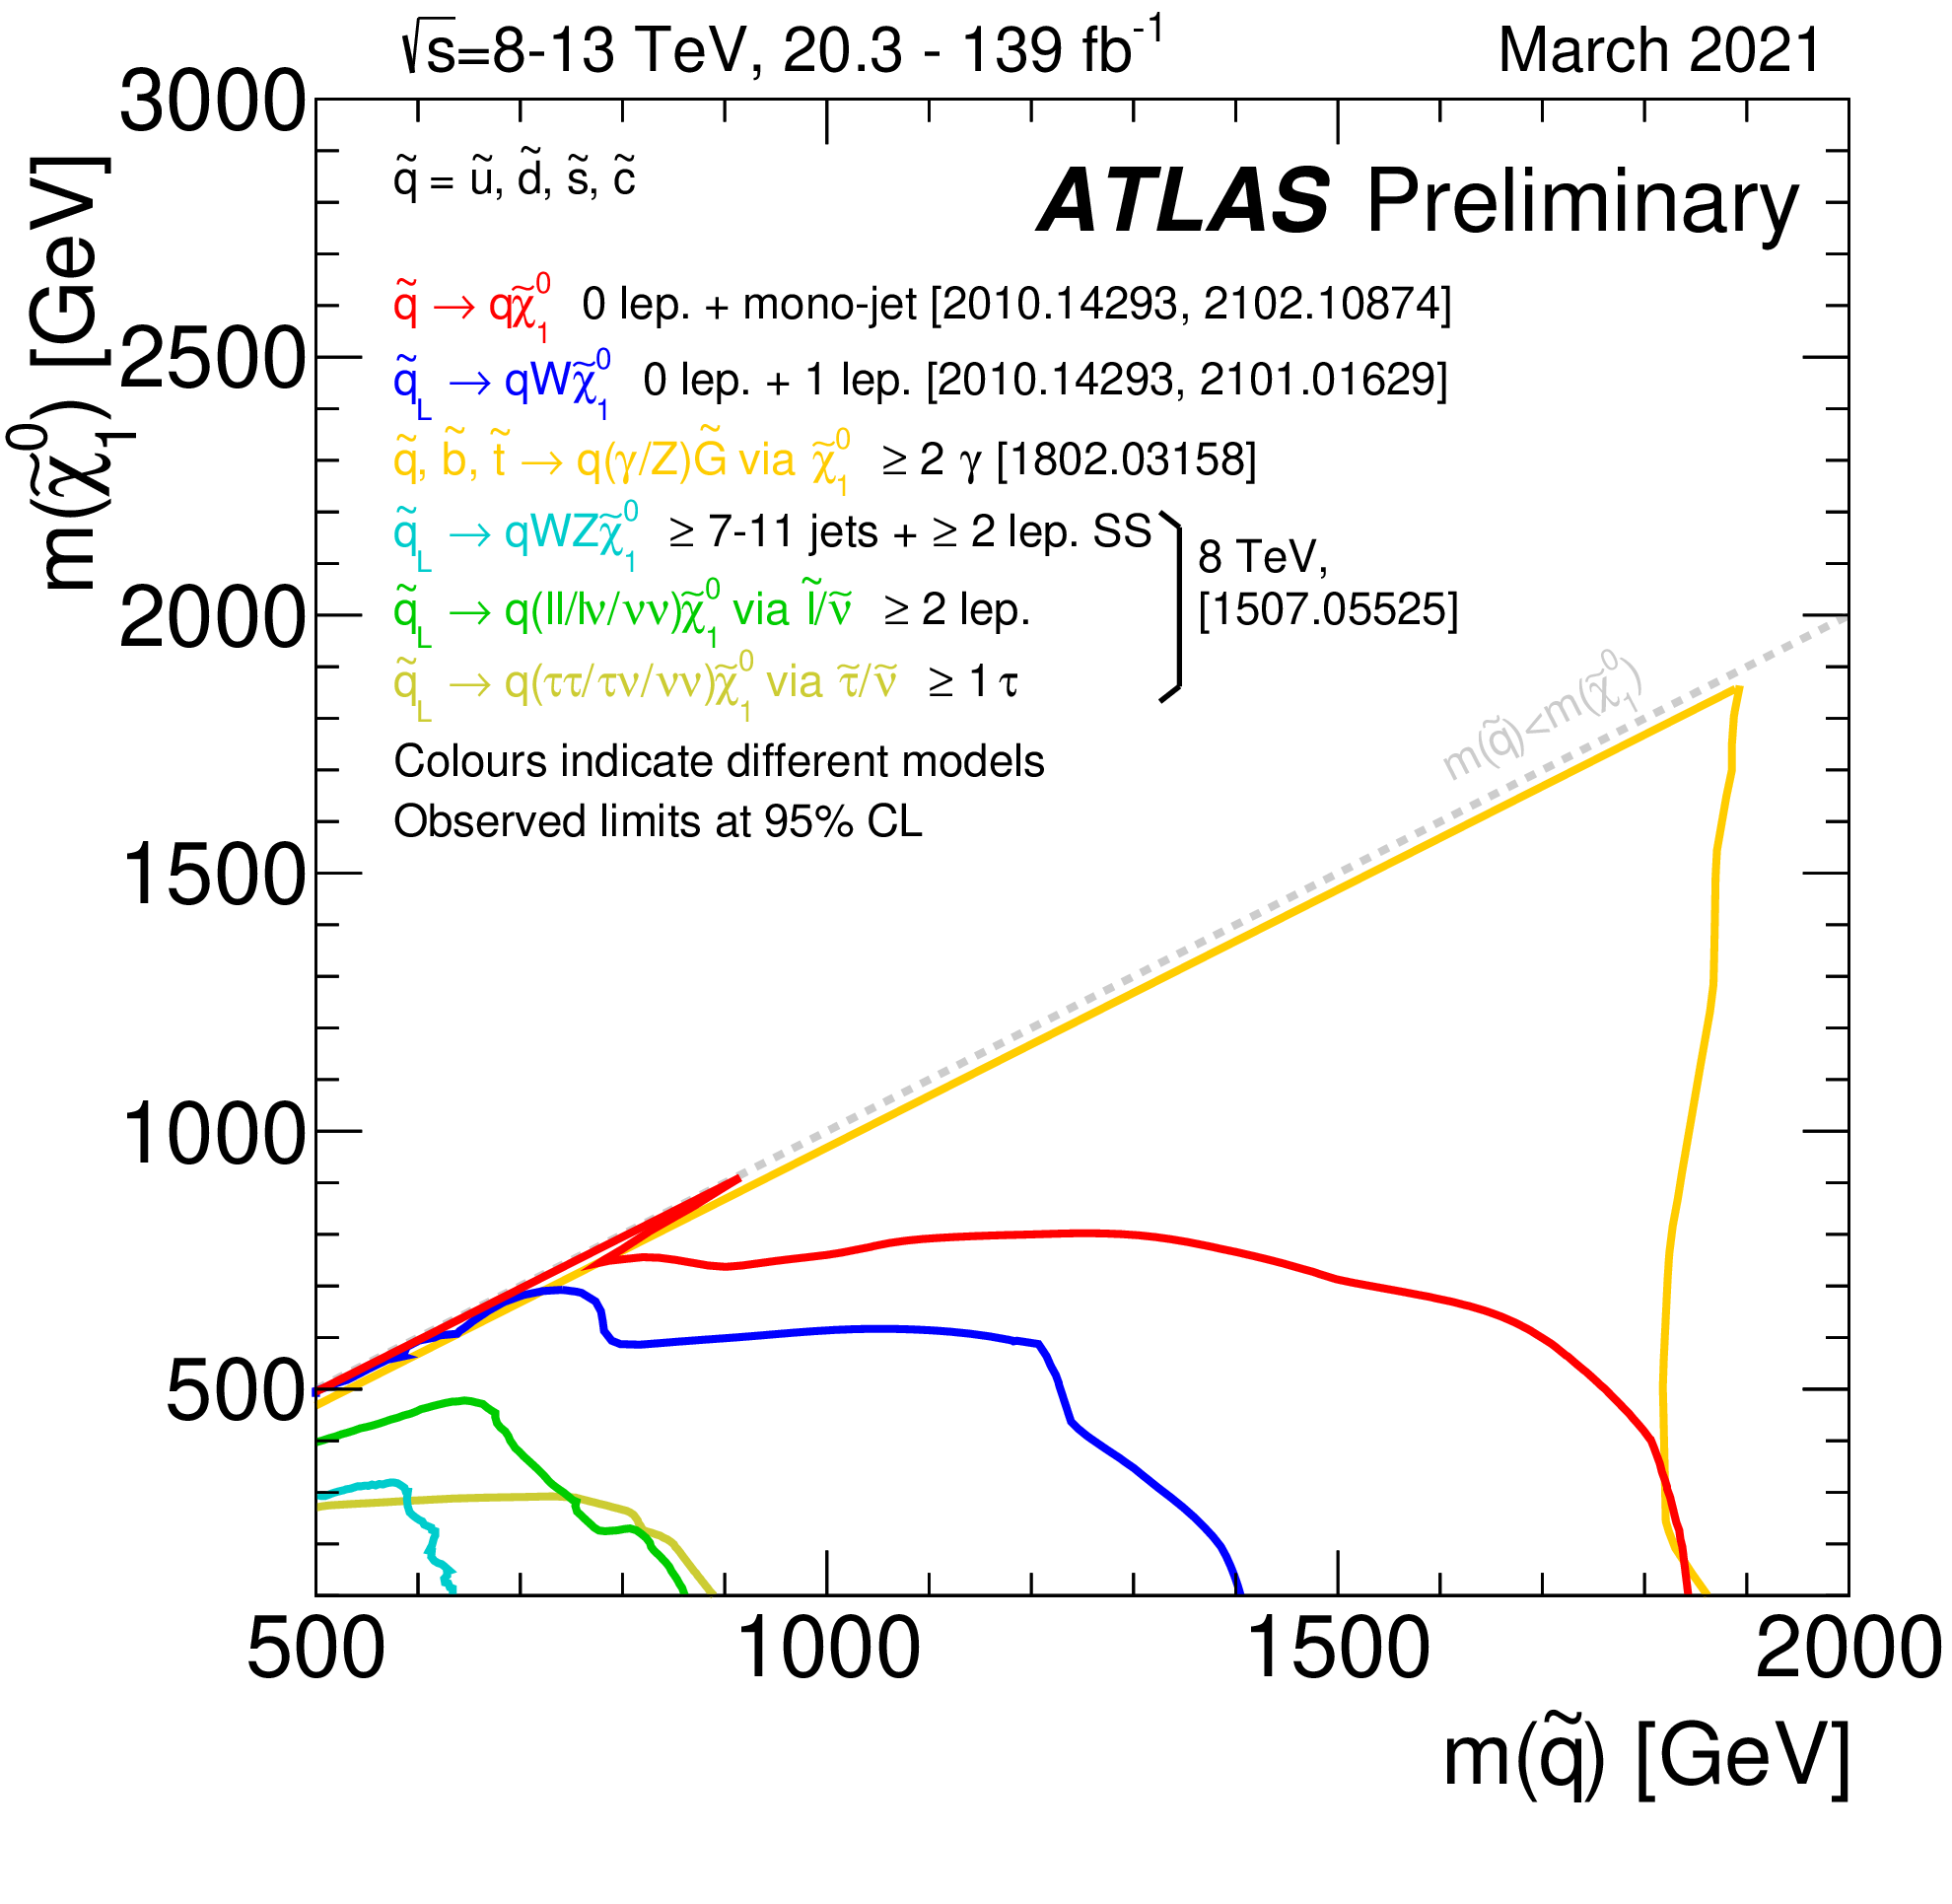
\includegraphics[width=0.49\textwidth]{figures/squark_limit} 
\caption{Excluded regions in the $(m_{\tilde g}, m_{\tilde\chi_1^0})$ (left) and $(m_{\tilde q},m_{\tilde\chi_1^0})$ (right) mass planes under different assumptions on the decays of the gluino and squarks \cite{ATL-PHYS-PUB-2021-019}. References for the individual analysis given in the figure.}
\label{fig:gluino_squarklimit}
\end{center}
\end{figure}
%%%

For the gluino the most minimal assumption we can make is that the gluino sheds its adjoint colour charge in the decay to two quarks of the first or second generation and a neutralino, $\tilde g \to q\bar q\tilde\chi_1^0$, either by a direct three-body decay or via an intermediary squark (red line).  We then get limits up to $m_{\tilde{g}}>2300$\,GeV under the assumption of a very light neutralino. This limit gradually weakens as the neutralino mass increases, and disappears beyond $m_{\tilde{\chi}_1^0}>1000$\,GeV for $m_{\tilde{g}}>1000$\,GeV. For $m_{\tilde{g}}<1000$\,GeV (not visible on the plot) most of the parameter space is excluded, with the exception that a small sliver remains when $m_{\tilde{g}} \simeq m_{\tilde{\chi}_1^0}$ in the degenerate scenario.

For the first two generations of squarks the most minimal decay is $\tilde q\to q\tilde\chi_1^0$. Here the bound (red) reaches to around $m_{\tilde q}>1800$\,GeV for a light neutralino, while for heavier neutralinos the bound disappears beyond $m_{\tilde{\chi}_1^0}>700-800$\,GeV for $m_{\tilde q}>800$\,GeV. Below a squark mass of around 800\,GeV most of the parameter space is excluded, but we again lose sensitivity when there is degeneracy between the squark and the neutralino. Here a search for mono-jets has some impact in closing the gap, which shows as a spike in the excluded region between 800 and 900\,GeV, however, despite poor visibility in the plot, a very degenerate squark--neutralino pair is still allowed below 800\,GeV. 

An additional assumption made in this plot is that all the eight squarks of the first two-generations are degenerate in mass and adding to the cross section. Should one squark generation or flavour be significantly lighter than the others this means a further reduction in the production cross section and thus a weaker bound. It is also fairly clear that removing R-parity, meaning that the LSP decays, also weakens the above conclusions due to the possible absence of significant missing energy. 


%\subsection{Sbottom}
%The above bounds on the first and second generation squarks do not apply to the third generation as they are generically lighter and can have more complicated decay signatures. In Fig.~\ref{fig:sbottom} we see current best limits from ATLAS on the lightest sbottom taken from~\cite{Aad:2013ija}. Note that this limit assumes 100\% branching ratio for $\tilde b_1\to b \tilde \chi_0^1$. If this branching ratio  is reduced to 60\% the excluded upper limit on the sbottom mass for $m_{\tilde\chi_1^0} < 150$\,GeV is reduced to 520 GeV. Similarly for $m_{\tilde b_1} = 250$\,GeV, the upper limit on $m_{\tilde\chi_1^0}$ is reduced by 30 GeV.
%
%\begin{figure}[h!]
%\begin{center}
%\includegraphics[scale=0.5]{figures/fig_05.eps} 
%\caption{Plot of the excluded area in the ($m_{\tilde{b}_1}$,$m_{\tilde{\chi}_1^0}$) plane. The limit from ATLAS is the red line, while the green and blue colored areas are excluded from different Tevatron experiments~\cite{Aad:2013ija}.\label{fig:sbottom}}
%\end{center}
%\end{figure}

%%%
\subsection{Stop}
For the stop there are many possible competing decay channels, meaning that limits set are rather model dependent. The two main decay categories for the lightest stop are decays via the chargino, $\tilde{t}_1\to b \tilde{\chi}^+_1$, a supersymmetrised version of the Standard Model $t\to bW^+$, and decays directly to the neutralino $\tilde{t}_1\to t\tilde{\chi}^0_1/ bW \tilde{\chi}^0_1/bff'\tilde\chi_1^0$, where $ff'$ represents the fermions in a $W$ decay, and where the dominant decay mode depends on the stop--neutralino mass difference. Since the chargino decay is also typically $\tilde{\chi}^+_1\to ff'\tilde\chi_1^0$, the experimental signature of stop production is $bff'\tilde{\chi}^0_1$, a mixture of missing energy, fermions that may either be leptons or result in jets, and a $b$-quark that forms a jet with distinct properties, called a $b$-jet.

%%%
\begin{figure}[t!]
\begin{center}
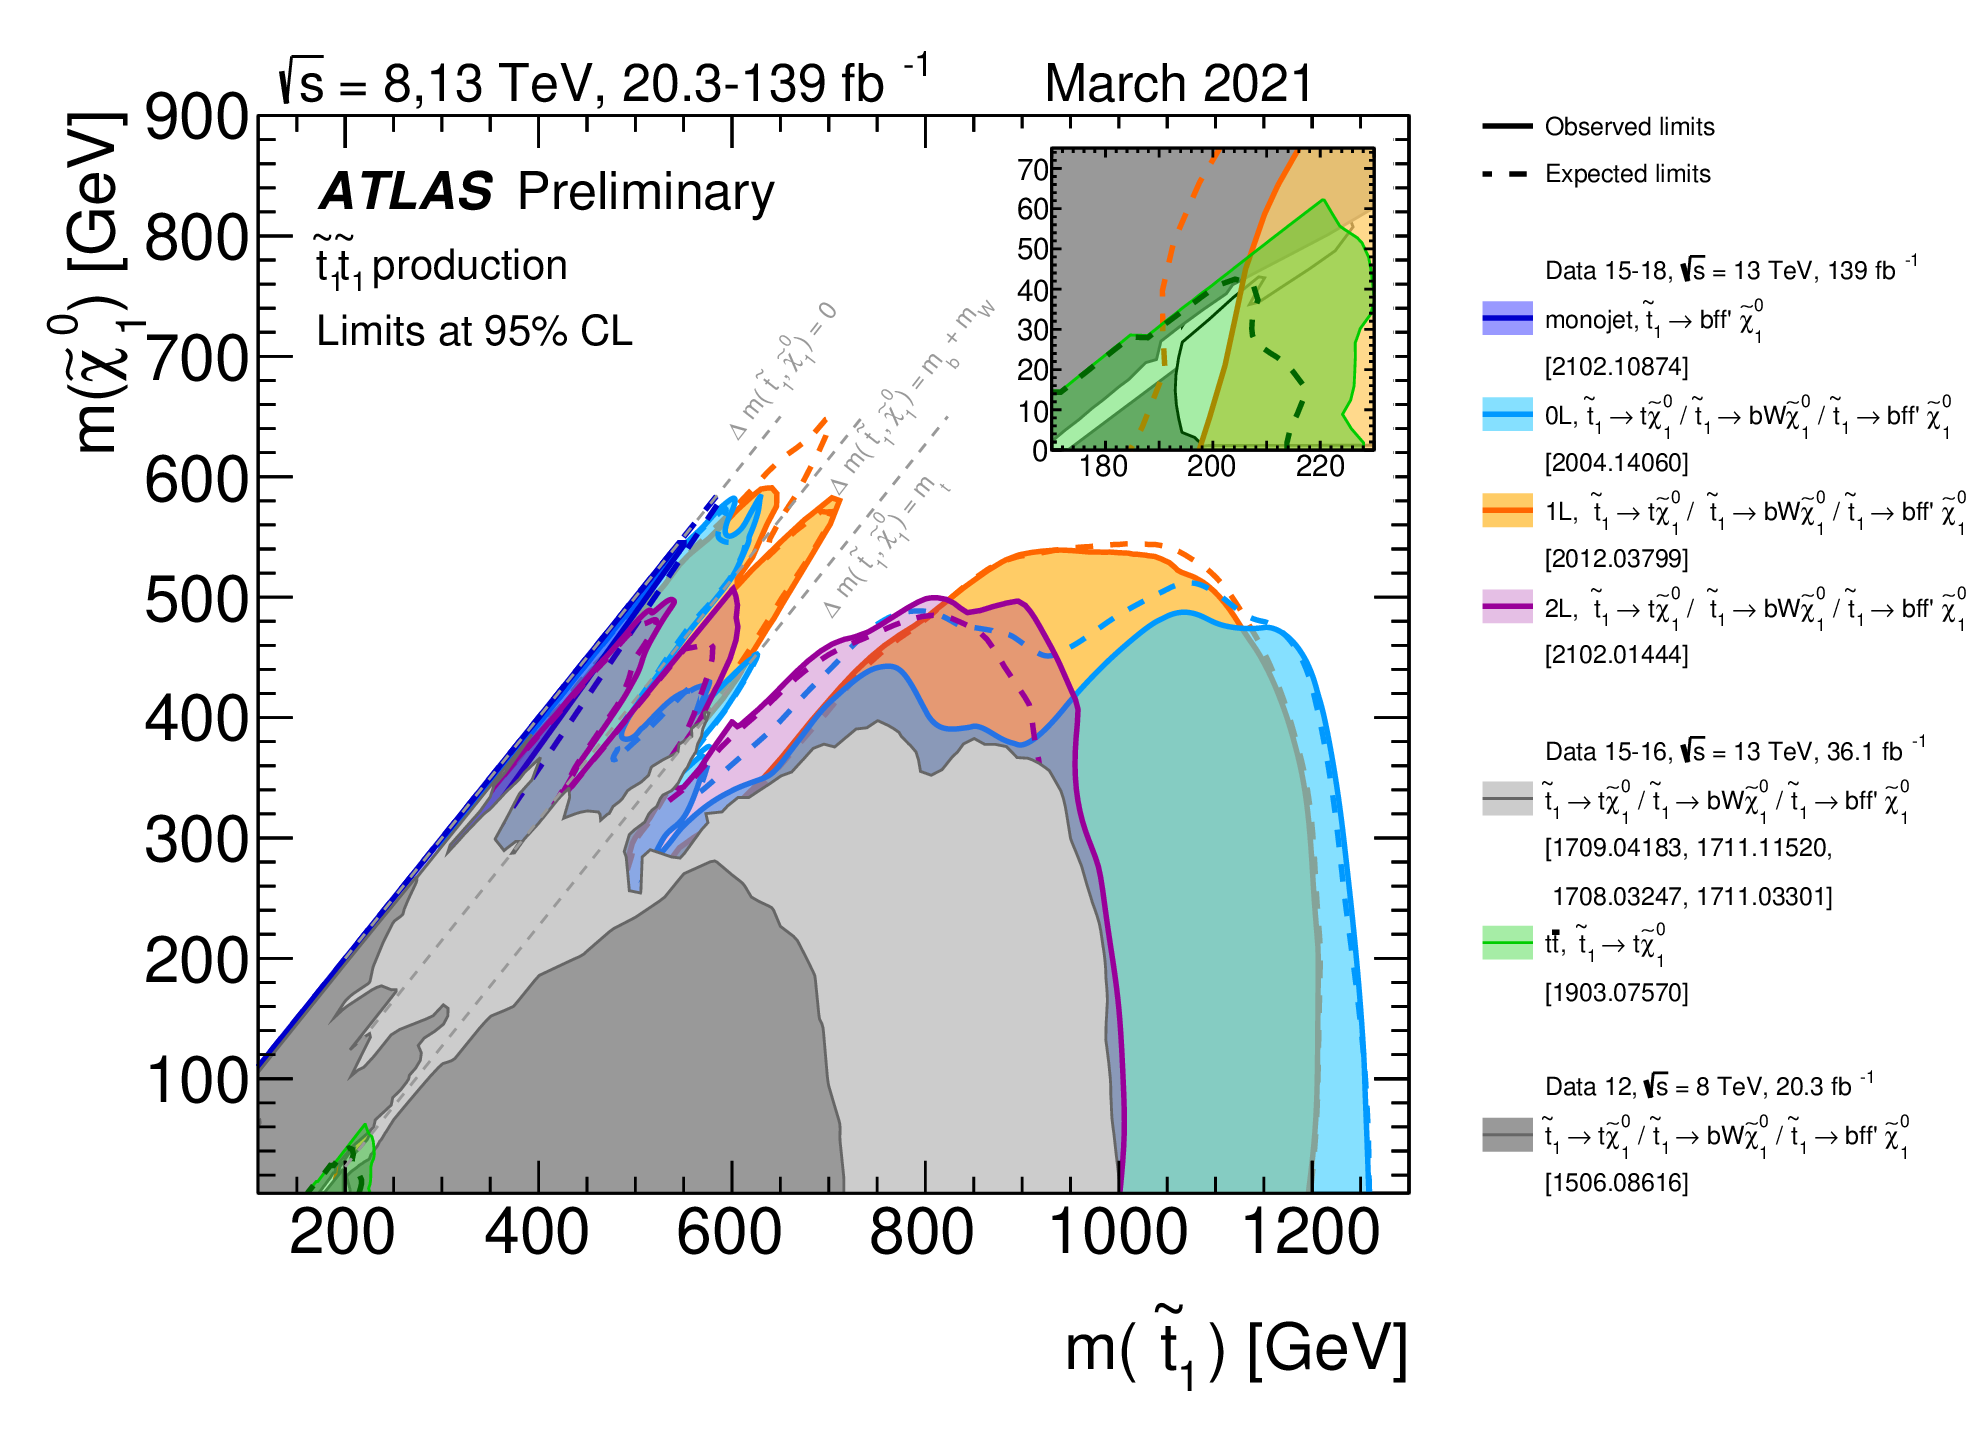
\includegraphics[width=\textwidth]{figures/stop_limit} 
\caption{Plot of the excluded area in the ($m_{\tilde{t}_1}$,$m_{\tilde{\chi}^0_1}$)  mass plane~\cite{ATL-PHYS-PUB-2021-019}. References for the individual analysis given in the figure.}
\label{fig:stoplimit}
\end{center}
\end{figure}
%%%

A summary of (the many) ATLAS searches for the stop is found in Fig.~\ref{fig:stoplimit} showing limits in the $(m_{\tilde t_1}, m_{\tilde\chi^0_1})$ mass plane. The dashed grey lines show the regions where the different stop decays are kinematically possible. We observe that for light neutralinos the limit goes all the way up to $m_{\tilde t_1}>1250$\,GeV, while there are essentially no limits for $m_{\tilde\chi^0_1} >580$\,GeV. Again degenerate scenarios 
have weaker bounds. When the stop approaches the neutralino plus top mass stop masses down to 600\,GeV are allowed. And, again not very visible, for a degenerate stop--neutralino the limit is virtually non-existent. As an additional complication, if the stop--neutralino mass difference is below the bottom quark mass, the standard stop decays no longer work and the flavour changing neutral current decay $\tilde{t}_1\to c\tilde{\chi}^0_1$ becomes dominant. This decay has multiple still open theoretical questions, both about the potentially long lifetime of the stop in this scenario, and exactly where in parameter space this transition occurs.


%%%
\subsection{Sleptons}
The mass bounds on sleptons will be very dependent on the assumed production mechanism. If the sleptons are produced indirectly in cascade decays from heavier squarks or gluinos they could have large cross sections, however, the most model independent bounds come from assuming only direct electroweak pair production through a virtual photon or $Z$.

%%%
\begin{figure}[t!]
\begin{center}
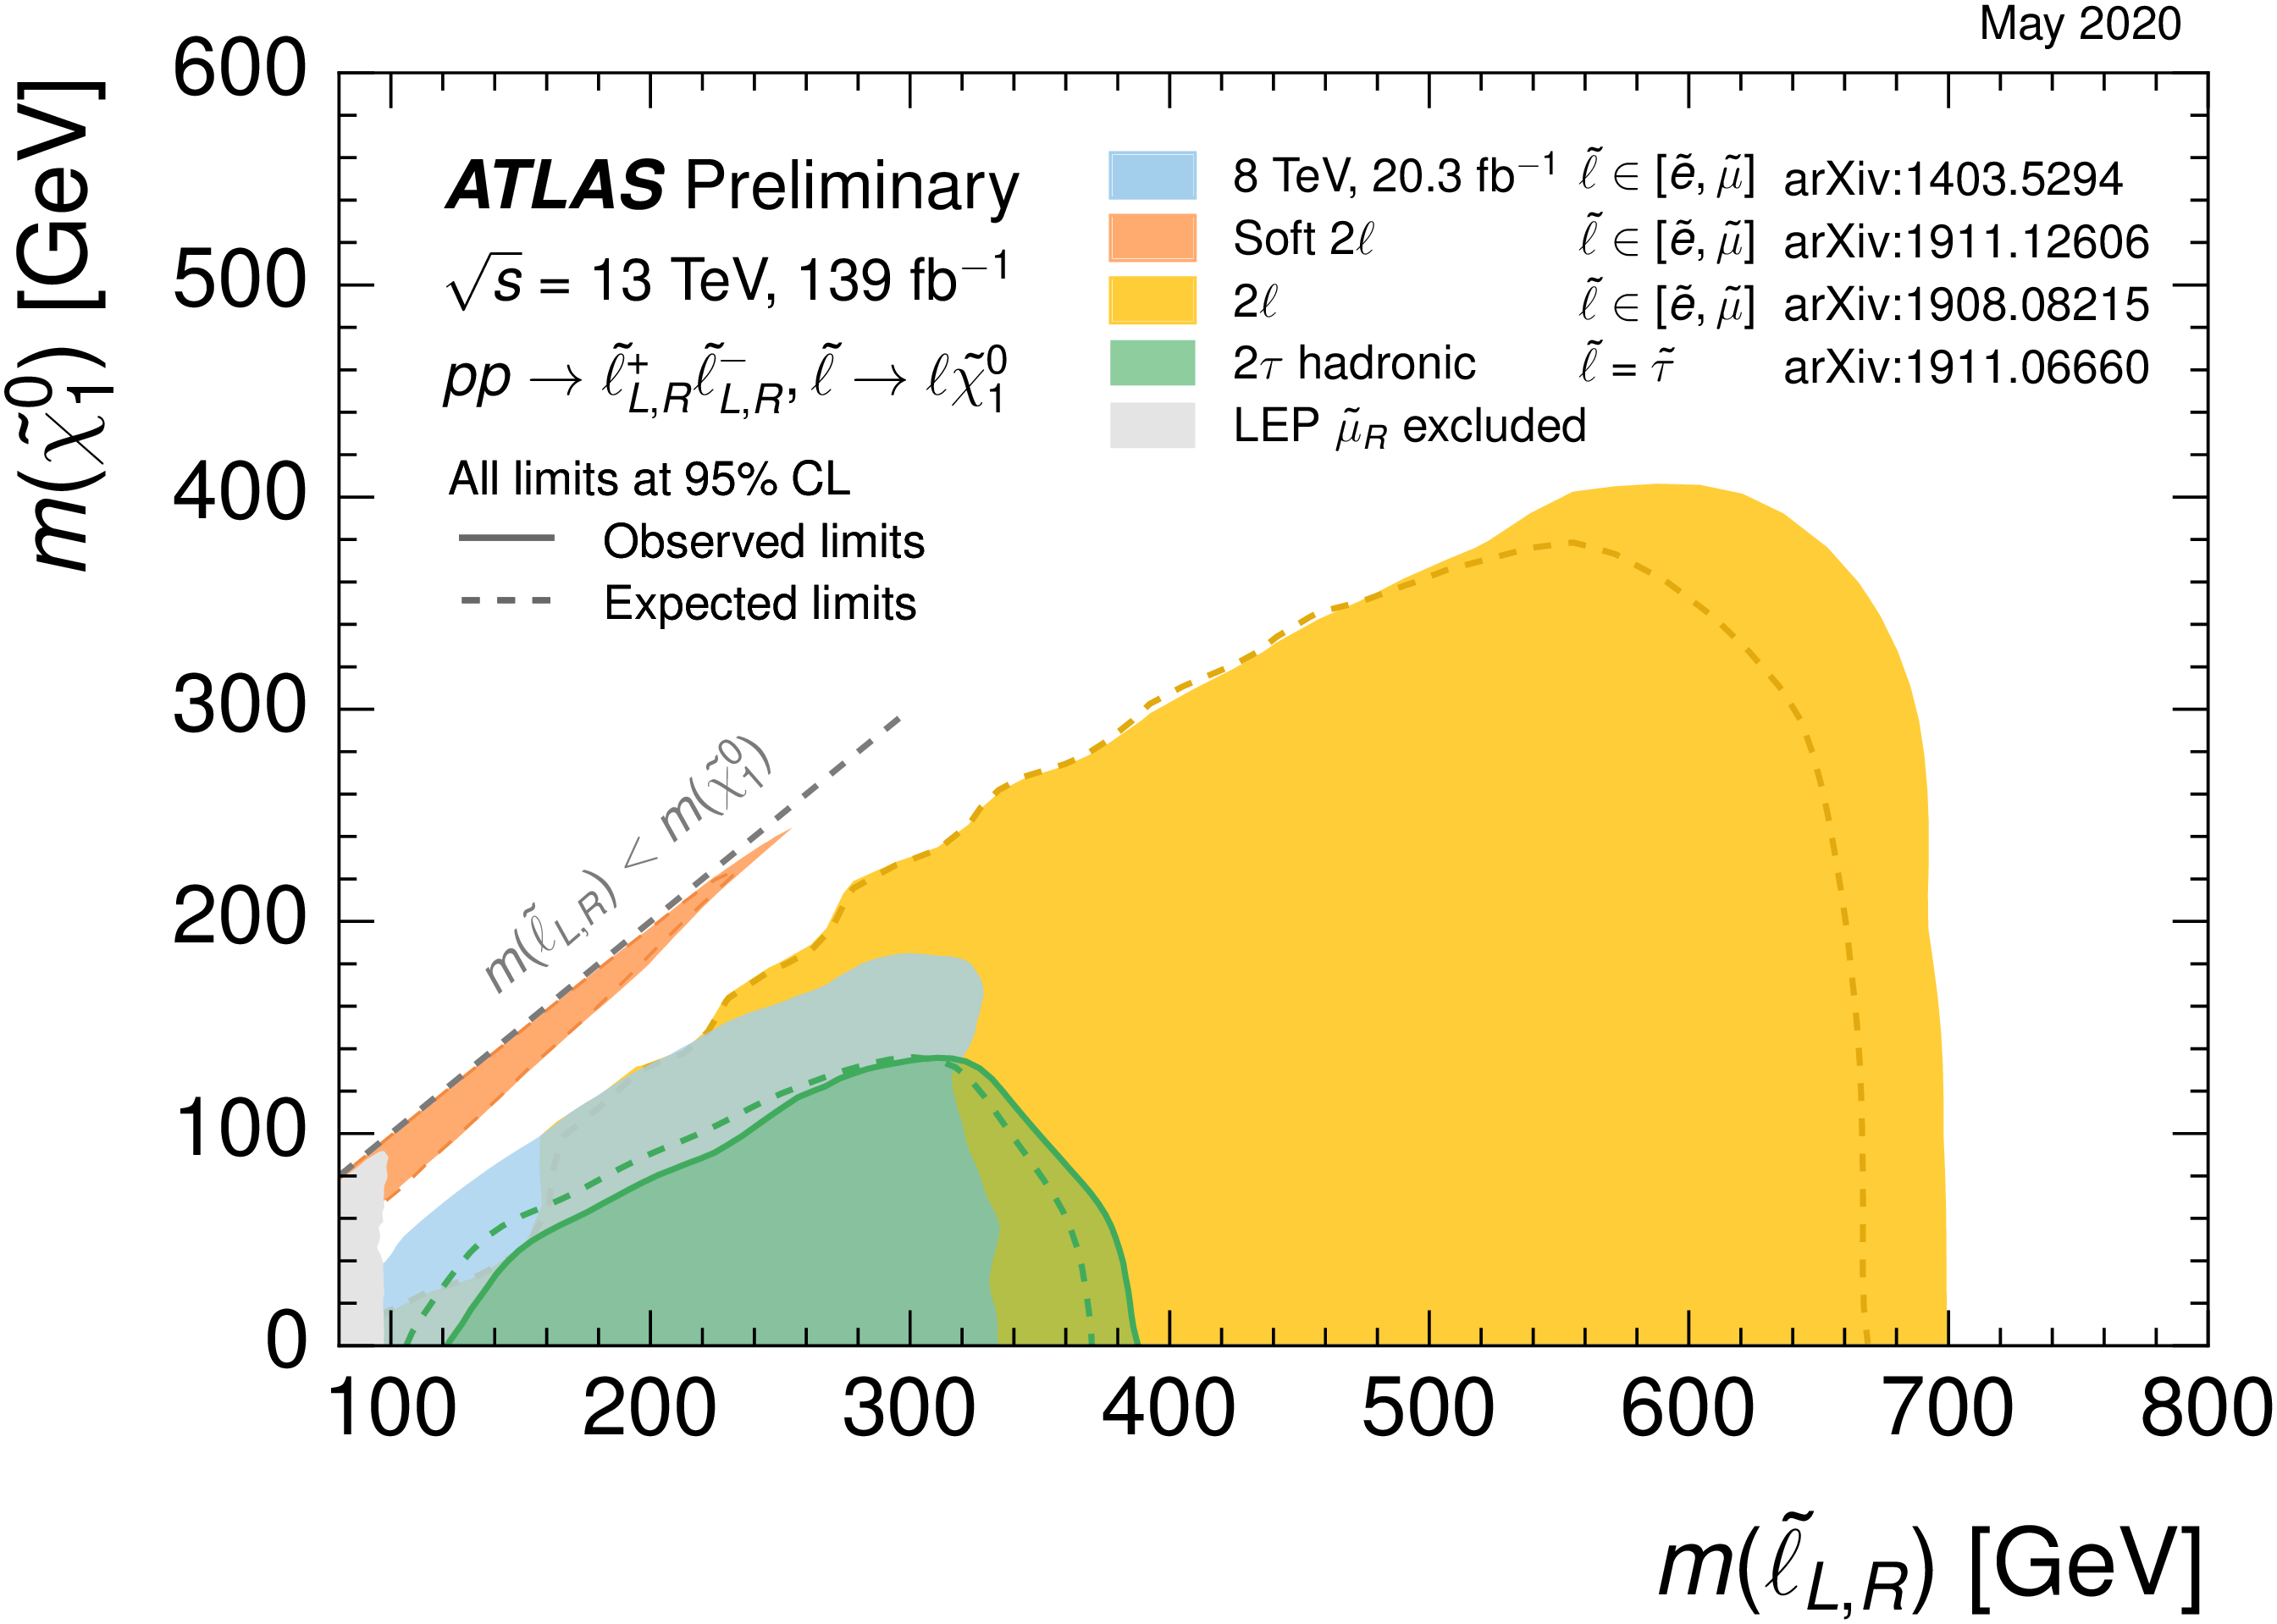
\includegraphics[width=0.95\textwidth]{figures/slepton_limit} 
\caption{Plot of the excluded area in the ($m_{\tilde l_{L,R}}$,\,$m_{\tilde\chi^0_1}$) plane for mass degenerate right- and left-handed  sleptons of different flavours~\cite{ATL-PHYS-PUB-2021-019}.}
\label{fig:sleptonlimit}
\end{center}
\end{figure}
%%%


The result for degenerate right- and left-handed charged sleptons from electroweak production, assuming decays with 100\% branching ratio to the lightest neutralino, are shown in Fig.~\ref{fig:sleptonlimit}. These limits separate between selectron and smuon production, and stau production. The former are assumed degenerate, and have stricter bounds than the stau, which is harder to reconstruct due to the many different possible tau decays involving extra neutrinos. For all slepton flavours we see that there is a gap in the mass plane down to very low masses where no sleptons are excluded, all the way down to masses below 100\,GeV where the LEP bound applies. This is yet another example of the problems with degeneracy. If the slepton--neutralino mass difference is around 50\,GeV and lower, it becomes difficult to reliably reconstruct the soft leptons from the slepton decay and to separate them from the ordinary Standard Model pair production of lepton pairs.


%%%
\subsection{Charginos and neutralinos}
As for the sleptons, bounds are dependent on the production process assumed. The search for direct electroweak pair production of the lightest neutralino, $\tilde{\chi}^0_1\tilde{\chi}^0_1$, has the same problem as at LEP, the coupling is vanishingly small for a non-higgsino $\tilde{\chi}^0_1$. This means that it is the heavier neutralinos and charginos that are typically searched for. Here some considerations on the possible masses hierarchies come into play. If the lightest neutralino is dominantly bino and the next-to-lightest dominantly wino ($M_1<M_2<|\mu|$) then the $\tilde{\chi}^0_2$ and $\tilde{\chi}^\pm_1$ states are degenerate in mass and the most important searches will be for $\tilde{\chi}^0_2\tilde{\chi}^\pm_1$ and $\tilde{\chi}^+_1\tilde{\chi}^-_1$ production.\footnote{Again because of the coupling in Eq.~(\ref{eq:ZNN_vertex}) the production of a pair of wino-like $\tilde{\chi}^0_2\tilde{\chi}^0_2$ is suppressed and the cross section is small.} These then decay as $\tilde{\chi}^0_2\to Z \tilde{\chi}^0_1$ or  $\tilde{\chi}^0_2\to h \tilde{\chi}^0_1$, and  $\tilde{\chi}^\pm_1\to W \tilde{\chi}^0_1$, where the bosons may be off-shell if the mass difference is small.
This is the scenario usually considered by the experiments, in part because winos give the largest electroweak production cross sections. 

%%%
\begin{figure}[t!]
\begin{center}
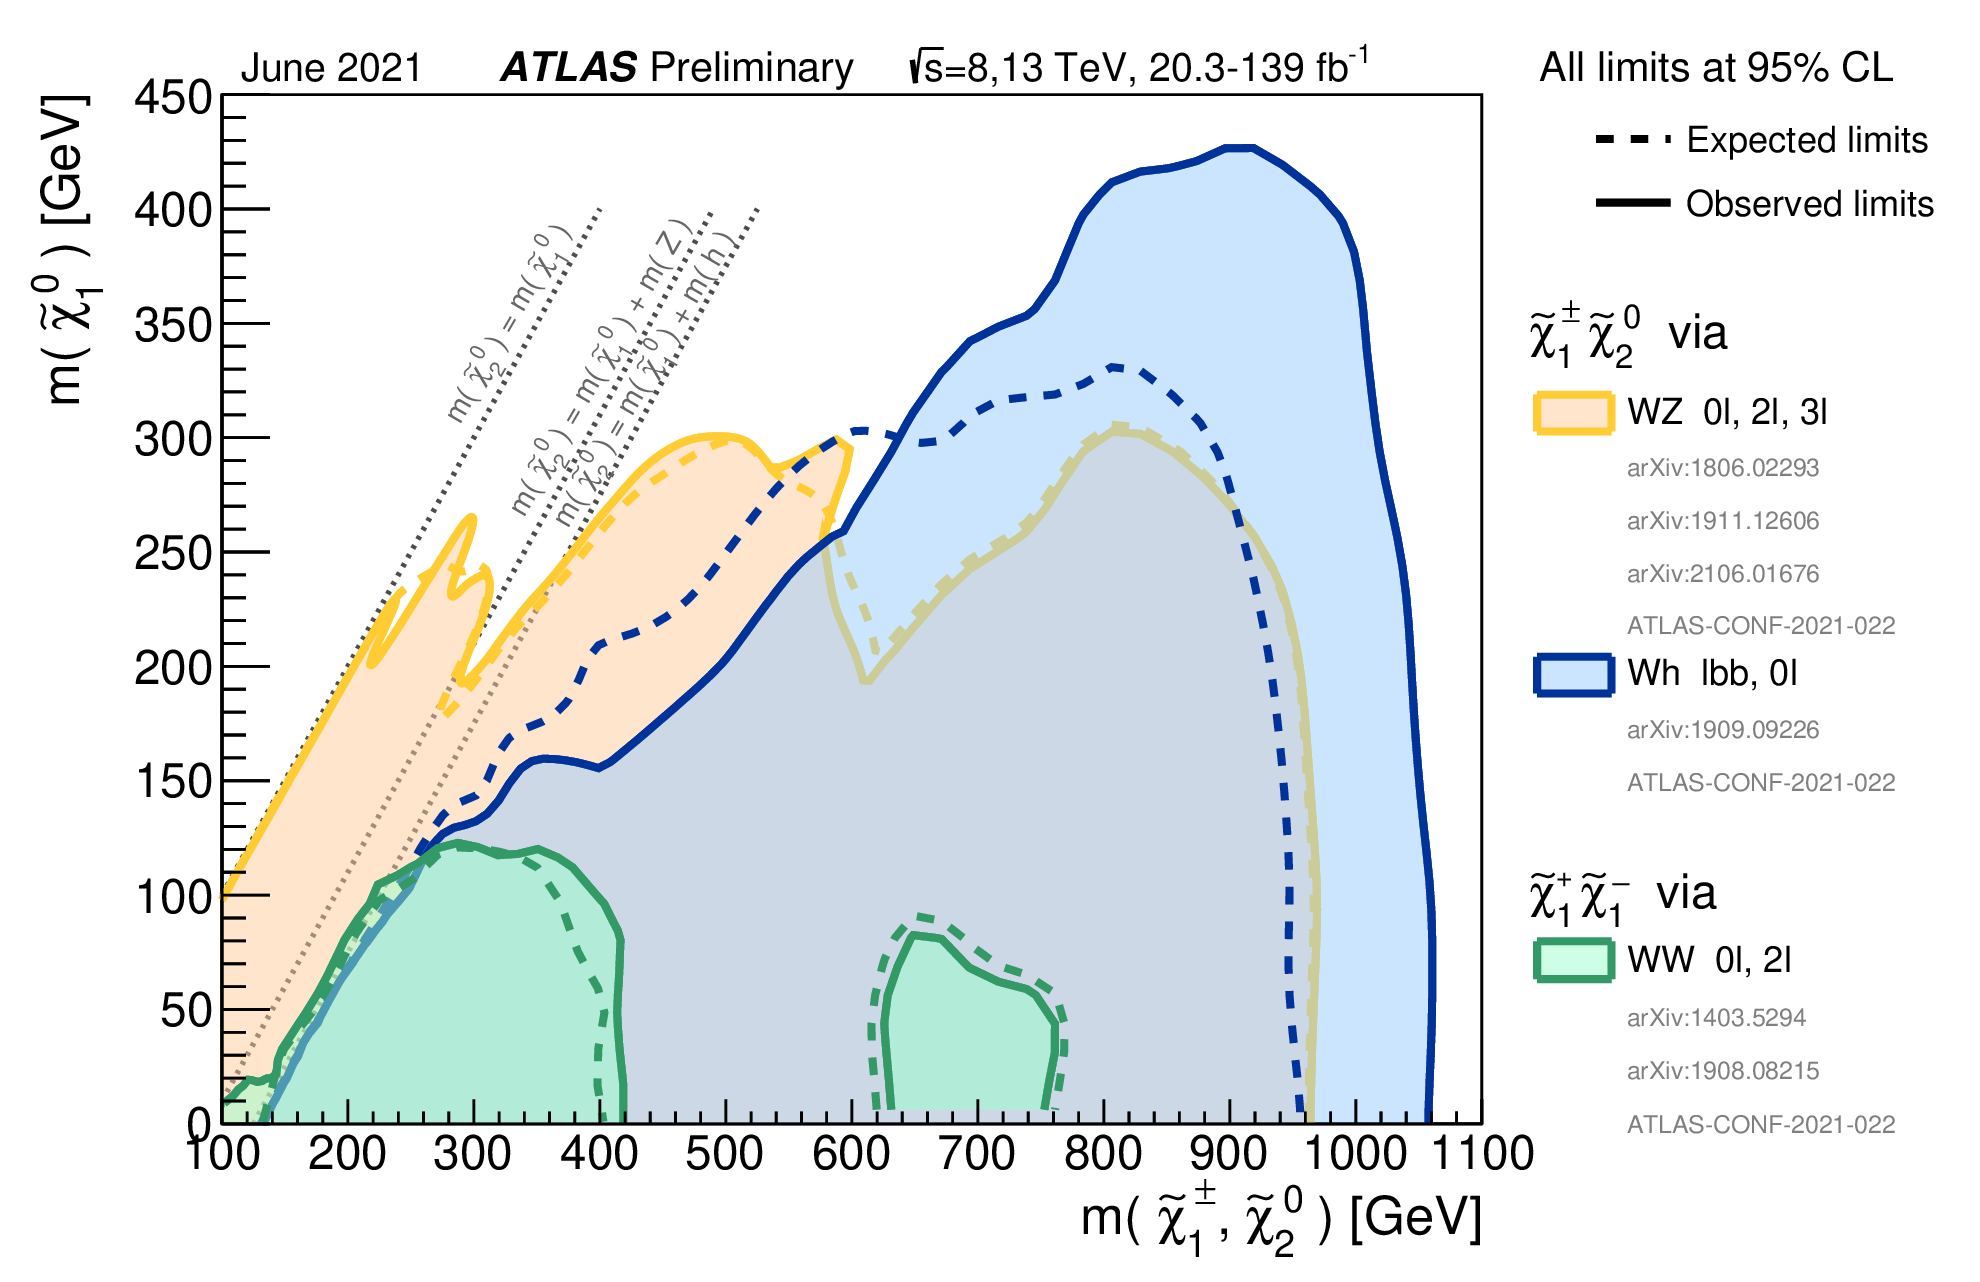
\includegraphics[width=0.9\textwidth]{figures/chargino_neutralino_limit} 
\caption{Plot of the excluded area in the ($m_{\tilde\chi_1^\pm,\tilde\chi_2^0}$,\,$m_{\tilde{\chi}^0_1}$) mass plane for different search signatures~\cite{ATL-PHYS-PUB-2021-019}. This plot assumes a degenerate wino-like  $\tilde{\chi}^0_2$ and $\tilde{\chi}^\pm_1$ and a 100\% branching ratio to the given decay channels.}
\label{fig:charginolimit}
\end{center}
\end{figure}
%%%

We show the current limits assuming degenerate wino-like states $\tilde{\chi}^0_2$ and $\tilde{\chi}^\pm_1$ in Fig.~\ref{fig:charginolimit}. We can see that limits up to 1050\,GeV can be set for $\tilde{\chi}^0_2$ and $\tilde{\chi}^\pm_1$ when the lightest neutralino is below around 200\,GeV. When the bosons in the decay go off-shell we see that the sensitivity of the searches go down significantly. If we move away from the wino-production scenario the production cross sections drop, and so does the reach of the experiments in the mass plane.

An additional important complication appears if the lightest neutralino is wino ($M_2<M_1,|\mu|$) or higgsino ($|\mu|<M_1,M_2$). Then the lightest neutralino and chargino, $\tilde{\chi}^0_1$ and  $\tilde{\chi}^\pm_1$ (for higgsinos also $\tilde{\chi}^0_2$), are degenerate, and the crucial question becomes how degenerate they are. If the mass difference is small but above around 300\,MeV, then the particles are very difficult to discover at all, despite potentially having very large cross sections if they are light. The decays of the produced $\tilde{\chi}^\pm_1$ (and for higgsinos $\tilde{\chi}^0_2$) into $\tilde{\chi}^0_1$ lead to very soft decay products, either leptons in $\tilde{\chi}^\pm_1\to \ell^\pm\nu_\ell\tilde{\chi}^0_1$ (and $\tilde\chi^0_2\to \ell^+\ell^-\tilde{\chi}^0_1$), or decays to pions (the lightest hadronic states) $\tilde{\chi}^\pm_1\to \pi^\pm\tilde{\chi}^0_1$ (and $\tilde\chi^0_2\to \pi^0\tilde{\chi}^0_1$), that are unobservable above the backgrounds of a hadron collider. 

If instead the mass difference becomes of the order off or less than the pion mass the width of the chargino can become so small that the state is sufficiently long lived to decay somewhere inside the detector, and not, effectively, at the interaction point. This would lead to charged tracks from the charginos that disappear somewhere inside the detector. Such disappearing track signatures are readily observable, and in fact the limits on very degenerate neutralinos and charginos are stronger than the limits on only somewhat degenerate ones.

The consequences of this complication is that it is very difficult to exclude near massless wino- or higgsino-like charginos and neutralinos at the LHC. However, since the chargino mass is constrained by the $Z$-width measured at LEP, there is an absolute lower limit of 45 GeV for both in this scenario. To improve significantly on this limit one may have to wait for a new lepton collider.


%%%%%%%%%%%%%%%%
\section{Precision observables}
%%%%%%%%%%%%%%%%
A different way to search for the signs of supersymmetric particles is their indirect effect on very accurately measured Standard Model particle properties and processes, so-called {\bf precision observables}, mostly through loop diagrams with sparticles. We will here discuss four different types of probes: the electroweak precision observables, the value of the anomalous magnetic moment of the muon $(g-2)_\mu$, the flavour changing neutral current (FCNC) process $b\to s\gamma$ and the very rare (and FCNC) process $B_s\to\mu\mu$.

%%%
\subsection{Electroweak precision observables}
%%%
When we talk about {\bf electroweak precision observables}, we study particle properties such as $M_W$ (or $M_Z$), $\Gamma_W$, $\Gamma_Z$, $m_t$ and $\sin\theta_W$, as well as the Higgs mass $m_h$ and the properties of the Higgs such as its couplings to all the other particles (gauge and Yukawa couplings) and its self-coupling. 

Up to 2012 we could study all of these as {\it functions} of the unknown Higgs mass, looking for deviations that could be a sign of for example supersymmetry. We show a fit of the Higgs mass to all available electroweak data and direct exclusion bounds in Fig.~\ref{fig:higgs_mass_prediction}, made by the Gfitter Collaboration in 2011 just before the LHC started taking significant amounts of data~\cite{Baak:2011ze}, a fit pretty much indicating that the most probable Standard Model Higgs mass was around 120 GeV.  Here, 
\[
\Delta\chi^2=\chi^2(m_h)-\min_{m_h}\chi^2(m_h),
\]
is the difference in the $\chi^2$ from the best fit point as a function of the Higgs mass, which has a standard interpretation in terms of $\sigma$s of significance for a one dimensional fit.

%%%
\begin{figure}[t!]
\begin{center}
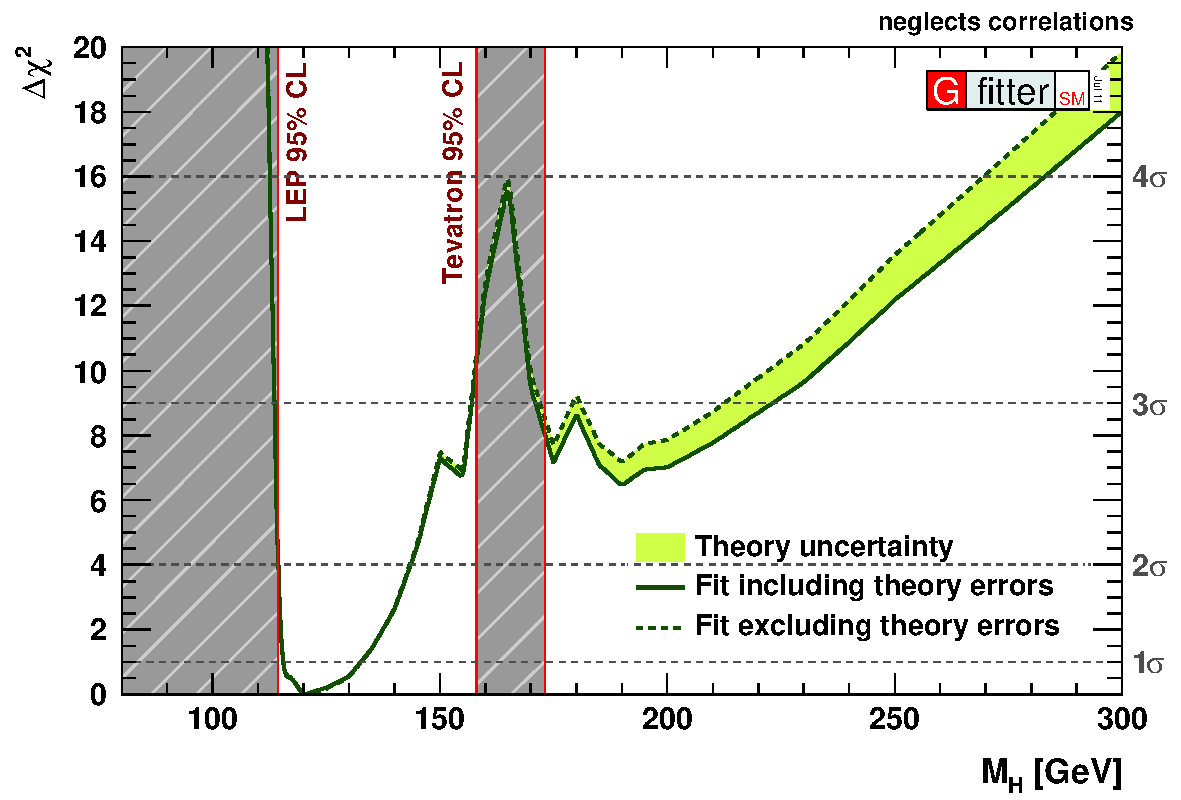
\includegraphics[width=\textwidth]{figures/higgs_mass_prediction} 
\caption{Plot of the total $\Delta \chi^2$ from all precision observable measurements and the direct exclusions bounds for the Standard Model Higgs set by LEP and the Tevatron, as a function of the Higgs mass~\cite{Baak:2011ze}.}
\label{fig:higgs_mass_prediction}
\end{center}
\end{figure}
%%%

Figure \ref{fig:mSUGRA_prediction} shows a similar plot for mSUGRA. At that time the absolute minimum of the fit, even taking into account the different number of parameters, gave a better fit for mSUGRA, $\min\chi^2_{\rm mSUGRA}<\min\chi^2_{\rm SM}$, but this changed quickly when the Higgs was found because of the position of the two minima.

%%%
\begin{figure}[h!]
\begin{center}
\includegraphics[width=0.7\textwidth]{figures/mSUGRApre.eps} 
\caption{Plot of the $\Delta \chi^2$ from all precision observable measurements for mSUGRA as a function of the Higgs mass. The yellow area shows the area excluded by LEP searches ({\it not} included in the fit), while the brown shows the theoretically inaccessible area.}
\label{fig:mSUGRA_prediction}
\end{center}
\end{figure}
%%%

Now all the parameters of the Standard Model -- neutrinos excepted -- have been determined to some precision. Thus the Standard Model is a completely constrained system. If we now do a electroweak fit the situation looks like that in Fig.~\ref{fig:EWfit_LHC2018}, where we show the global fit to all measurements {\it except} the top and $W$ masses, compared to the measured values of the $W$ and top masses. Clearly what we are seeing here is (still?) consistent with the Standard Model.

%%%
\begin{figure}[h!]
\begin{center}
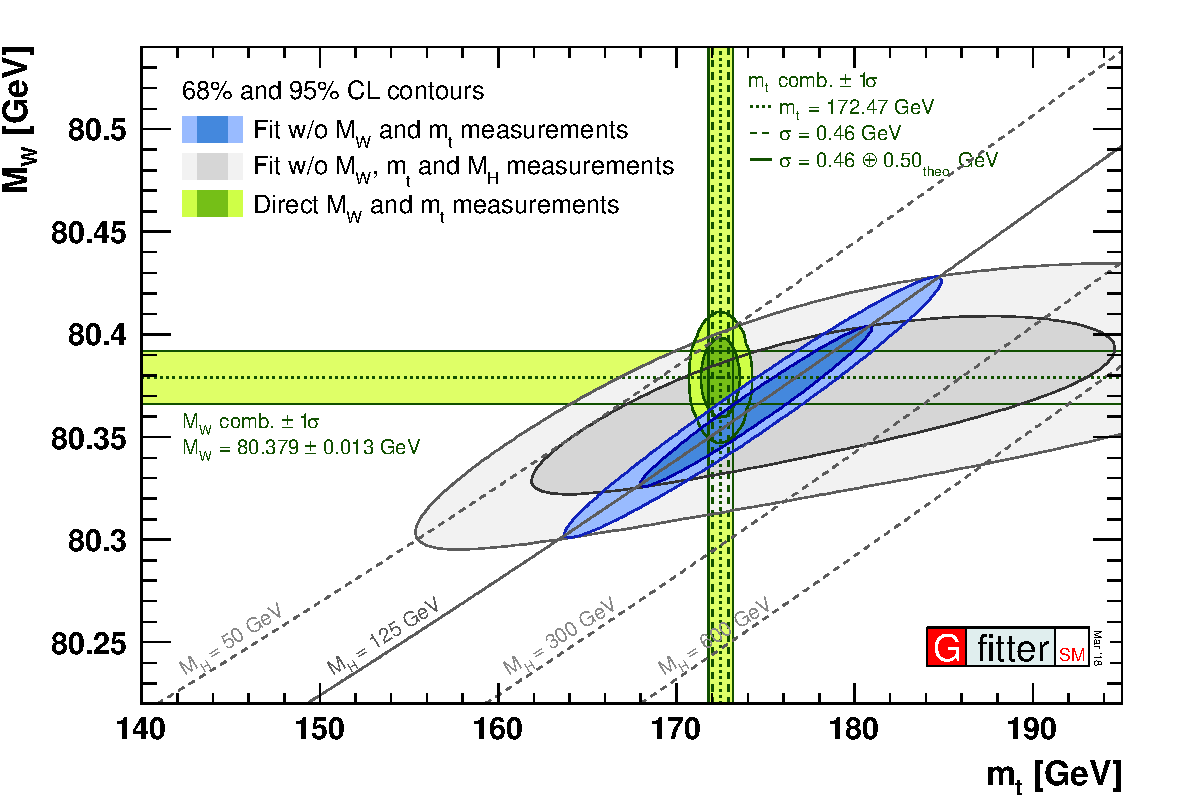
\includegraphics[width=0.85\textwidth]{figures/MW_vs_mt} 
\caption{Electroweak fit excluding $M_W$ and $m_t$ (blue), compared to their measured values (green)~\cite{Haller:2018nnx}.}
\label{fig:EWfit_LHC2018}
\end{center}
\end{figure}
%%%


%%%
\subsection{$(g-2)_\mu$}
%%%
The {\bf anomalous magnetic moment} of the muon, $g_\mu$, in effect the interaction of a muon with an external electromagnetic field shown in Fig.~\ref{moudig} a), was calculated by Dirac in relativistic quantum mechanics as $g_\mu=2$. However, in quantum field theory we have higher order corrections from loop-process such as shown in  Fig.~\ref{moudig} b), that makes $g_\mu$ deviate from two. 

It was very precisely measured by the E821 experiment at BNL \cite{Bennett:2006fi} to be:
\[g_\mu^\text{exp} = 2.00116592089(63),\]
or, in terms of the deviation $a_\mu=g_\mu-2$,
\[a_\mu^\text{exp}=11659208.9(6.3)\cdot 10^{-10},\]
where the parenthesis indicates the uncertainty on the last digits. 

In the Standard Model we find the prediction
\[a_\mu^\text{SM}=11659183.0(5.1)\cdot 10^{-10},\]
giving a difference with respect to the experimental value of
\[\Delta a_\mu \equiv a_\mu^{\rm exp}-a_\mu^{\rm SM} = (25.9\pm 8.1)\cdot 10^{-10},\]
a value which is 3.2$\sigma$ away from zero. Recently, the Muon g-2 Collaboration at Fermilab made a new measurement~\cite{Muong-2:2021ojo} confirming this discrepancy with the value
\[\Delta a_\mu = 25.1\pm 5.9\cdot 10^{-10},\]
corresponding to $4.2\sigma$. The Muon g-2 Collaboration is set to make further improvements on this number, expecting to reduce the uncertainty by a factor of $2-4$.

However, we should be aware that some of the Standard Model contributions involve hadronic loops, {\it e.g.} the so-called {\bf hadronic vacuum polarisation} shown in Figure~\ref{moudig} b), where one has to rely on experimental information from low energy $e^+e^-\to \gamma^* \to {\rm hadrons}$ in order to estimate a contribution of $a_\mu^{\rm HVP}=10.5(2.6)\cdot 10^{-10}$, which is of the same order of magnitude as the discrepancy, and may be prone to errors in the interpretation. 

%%%
\begin{figure}[h!]
\begin{center}
\includegraphics{figures/muonprec.eps} 
\caption{Diagrams for muon interaction with an electromagnetic field. Loop corrections to the tree level diagram a) give the value of $a_\mu$. Diagram b) shows hadronic vacuum polarization where the blob contains QCD fields. Diagrams c) and d) show the lowest order MSSM contributions to $a_\mu$.}
\label{moudig}
\end{center}
\end{figure}
%

In the MSSM we can have contributions to $a_\mu$ at the one-loop level, either by the exchange of one of the new Higgs bosons across the muon line, or by loops containing a smuon $\tilde\mu$ or muon-sneutrino $\tilde\nu_\mu$, together with a neutralino or chargino. The diagrams for the latter two processes are shown in Figure~\ref{moudig} c) and d). These contribute opposite sign terms $a_\mu(\tilde{\chi}^0)$ and $a_\mu(\tilde{\chi}^-)$. A thorough analysis shows that we need $\mu>0$ in order to give a positive contribution that will close the gap between the experimnetal value and the prediction. In order to get a sufficiently large contribution the loop masses must be less than $500-600$\,GeV for $\tan\beta = 40-50$ and $200-300$\,GeV for $\tan\beta \simeq10$. However, as we saw in Sec.~\ref{sec:current_LHC_bounds} this is not implausible.


%%%
\subsection{$b \to s\gamma$}
%%%
The  quark level process $b \to s\gamma$ is a Flavour Changing Neutral Current (FCNC) process which must proceed through loops in the Standard Model since there are no tree-level FCNC interactions there. At meson level it leads to measurable decays of the type $B\to X_s\gamma$, where $X_s$ is some meson with a strange quark, {\it e.g.}\  the decay $B\to K\gamma$. Figure~\ref{btosdiags} a) shows the one-loop Standard Model contribution with a virtual $W$ and up-type quarks. This contribution is suppressed by the smallness of the CKM entries in the $W$-vertices which favours diagrams with a top quark in the loop, and the large masses, $M_W$ and $m_t$, in the loop.

%%%
\begin{figure}[h!]
\begin{center}
\includegraphics[width=\textwidth]{figures/btosdiags.eps} 
\caption{Diagrams for the process $b \to s\gamma$. a) shows the SM diagram while b), c) and d) show MSSM contributions.\label{btosdiags}}
\end{center}
\end{figure}
%%%

The process has been calculated at next-to-next-to-leading order (NNLO) in the Standard Model to be ${\rm Br}(B\to X_s\gamma)_{\rm SM} = (3.36 \pm 0.23)\cdot 10^{-4}$ for $E_\gamma \geq 1.6$\,GeV~\cite{Misiak:2015xwa,Czakon:2015exa}, inclusively summing over all meson final states.\footnote{For the process $b\to d \gamma$ the Standard Model calculation yields  ${\rm BR} (B \to X_d \gamma) = 1.73^{+0.12}_{-0.22} \cdot 10^{-5}$.}

Supersymmetry may contribute to this process, {\it e.g.} with diagrams such as Fig.~\ref{btosdiags} b) where the  $m_{bs}^2\tilde{b}^*\tilde{s}$ mass term that changes a $\tilde b_1$ to a $\tilde s$ is a soft breaking off-diagonal term, often denoted $\delta_{23}$. The main MSSM contributions are expected to come from chargino--stop\footnote{We usually expect a higher generation off-diagonal terms to be larger due to RGE running controlled by Yukawa couplings.} and charged higgs--top loops, as shown in Figs.~\ref{btosdiags} c) and d), respectively. However,  there is little room for effects from superymmetry  since the current experimental world average is ${\rm Br}(B\to X_s\gamma)=(3.32\pm 0.15)\cdot 10^{-4}$ (PDG 2010). This means that either the charged Higgs is heavy enough and the stop-scharm soft mass term small enough, or that there are cancellations between the contributions. 


%%%
\subsection{$B_s \to \mu^+\mu^-$}
%%%
The process  $B_s \to \mu^+\mu^-$ is another FCNC process as either the bottom or the strange quark must change flavour in order to couple to the muons. The SM process is shown in Fig.~\ref{bsmudiags} a), involving an intermediary $Z$-boson. There is additional suppression from a CKM factor in one of the $W$-vertices, in order to change a third generation quark to a second generation quark, or {\it vice versa}. On top of this, it also suffers from what is called {\bf helicity suppression} in the SM. The $Z$-boson is spin-1, while the starting point meson $B_s$ is spin-0 (pseudoscalar), meaning that the spins of the quarks are opposite. At some point in the diagram the helicity (chirality) must ``flip". This introduces an extra suppression proportional to $m_\mu^2/M_{B_s}^2$, making the expected rate extremely small and sensitive to supersymmetry contributions. We get a similarly supressed process for $B_d$ with a $\bar d$-quark instead of the $\bar s$ in the initial state.

\begin{figure}[h!]
\begin{center}
\includegraphics[clip=true,width=0.45\textwidth,trim=0 4.2cm 0 0]{figures/bsmudiag.eps} 
\includegraphics[width=0.45\textwidth]{figures/pmssm2.eps} 
\caption{Diagrams for the process $B_s \to \mu^+\mu^-$. Diagram a) shows one of the leading SM contributions, while b) shows one contribution from the MSSM taken from~\cite{Bobeth:2001sq}. \label{bsmudiags}}
\end{center}
\end{figure}

The predicted SM branching ratios for these processes are~\cite{Bobeth:2013uxa}:
\begin{eqnarray}
{\rm Br}(B_s \to \mu^+\mu^-) &=& (3.65 \pm 0.23)\cdot 10^{-9},\\
{\rm Br}(B_d \to \mu^+\mu^-) &=& (1.06 \pm 0.09)\cdot 10^{-10}.
\end{eqnarray}
First evidence for the $B_s$ decay was shown by the LHCb collaboration in 2012. The final observation required combining Run I data from both LHCb and CMS, and was published in 2014~\cite{CMS:2014xfa}. The current values are:
\begin{eqnarray}
{\rm Br}(B_s \to \mu^+\mu^-) &=&  2.8^{+0.7}_{-0.6}\cdot 10^{-9},\\
{\rm Br}(B_d \to \mu^+\mu^-) &=&  3.9^{+1.6}_{-1.4}\cdot 10^{-10},
\end{eqnarray}
where one should keep in mind that the $B_d$ decay has only evidence at $3.2\sigma$ significance.

In the MSSM there are contributions from process such as shown in Fig.~\ref{bsmudiags} b). These contributions are proportional to $\tan^6\beta$, which makes the decay process highly sensitive to scenarios with large $\tan\beta$. To see this dependence, notice that $\mu$ couples to the mediating heavy higgses $H/A^0$ through the Yukawa term $y^l_{22} L_2 H_d \overline{E}_2$ in the superpotential, and the Yukawa constant in this term, $y^l_{22} = y_\mu$, is connected to the fermion mass through $m_\mu = y_\mu v\cos\beta$. Thus this vertex is proportional to $1/\cos\beta$ or $\tan\beta$, giving a factor $\tan^2\beta$ in the amplitude squared.\footnote{Remember that in the limit of large $\tan\beta$
\begin{equation}
\cos\beta= \pm \frac{1}{\sqrt{1+\tan^2\beta}}= \pm \frac{1}{\tan\beta\sqrt{1+\frac{1}{\tan^2\beta}}}\simeq\pm \frac{1}{\tan\beta}.
\end{equation}
}

Furthermore, a chargino(higgsino)--stop loop can couple the strange and bottom quarks to the higgs. These couplings are proportional to the bottom Yukawa coupling $y_b$, from the superpotential terms $y_{33}^dQ_3H_d\bar D_3$, which appears in the stop--chargino--bottom vertex, and the  $y_{32}^uQ_3H_d\bar D_2$, which appears in the strange--chargino--stop vertex. Both these Yukawa couplings are proportional to $y_b$ and thus to  $1/\cos\beta$, giving a further factor of $\tan^4\beta$ in the amplitude squared. This $\tan\beta$ dependence makes $B_s \to \mu^+\mu^-$ an excellent channel for  discovering supersymmetry, and puts very stringent bounds on the sparticle masses in large $\tan\beta$ scenarios.


%%%%%%%%%%%%%
\section{Excercises}
%%%%%%%%%%%%%

\begin{Exercise}[]
From relativistic kinematics, show Eq.~(\ref{eq:m_ab}). {\it Hint:} the choice of rest frame is very important in order to simplify the calculation.
\end{Exercise}

\begin{Exercise}[]
Find the total cross section for the process $q\bar{q} \rightarrow \tilde{q}\tilde{q}^*$ via an s-channel gluon shown in Fig.~\ref{fig:feynmanq}.
%%%
\begin{figure}[h!]
\begin{center}
\unitlength=1mm
\begin{fmffile}{feynman_qqgqq}
\begin{fmfgraph*}(40,20)
  \fmfleft{i1,i2}
  \fmfright{o1,o2}
  \fmf{fermion}{i2,v1,i1}
  \fmf{gluon, label=$g$, label.dist=0.08w}{v1,v2}
  \fmf{dashes}{o1,v2,o2}
  \fmflabel{$\bar{q}_j^s, p$}{i1}
  \fmflabel{$q^r_i, k$}{i2}
  \fmflabel{$\tilde{q}_m, k'$}{o2}
  \fmflabel{$\tilde{q}^*_n, p'$}{o1}
  \fmflabel{$\mu$}{v1}
  \fmflabel{$\nu$}{v2}
  \fmfdot{v1}
  \fmfdot{v2}
\end{fmfgraph*}
\end{fmffile}
\vspace{5mm}
\caption{Strong production of a squark--anti-squark pair through a gluon.}
\label{fig:feynmanq}
\end{center}
\end{figure}
%%%
\end{Exercise}

\begin{Answer}
We will in the following take all outgoing momenta to go out of the vertex. The indices $abcd$ are gluon indices ($1,...,8$), $rs$ are spin indices ($1,2$), and $ijmn$ are colour indices ($1,2,3)$. The relevant  Feynman rules are as follows:
\begin{itemize}
\item Incoming quark: $u^r(k)$.
\item Incoming antiquark: $\bar{v}^s(p)$.
\item Gluon propagator: $-i \frac{g_{\mu\nu}}{s}\delta^{ab}$.
\item Vertex $q \bar{q} g$: $- i t^a_{ij}\gamma^\mu g_s$.
\item Vertex $\tilde{q}\tilde{q}^* g$: $- i t^b_{mn} (k'-p')^\nu g_s$.
\end{itemize}
We will assume the SM particles to have negligible mass compared to the squarks.

The matrix element is then given as
\begin{equation*}
\mathcal{M} = -\frac{g_s^2}{s} t^a_{ij} t^b_{mn} \delta^{ab} \bar{v}^s\gamma^\mu u^r(k'-p')_\mu.
\end{equation*}

In the squared amplitude we average over all incoming spin and colour, and sum over the outgoing:
\begin{align*}
|\bar{\mathcal{M}}|^2 & = \frac{1}{4}\cdot \frac{1}{9} \frac{g_s^4}{s^2}\sum_{ab}\sum_{cd}\sum_{rs}\sum_{ijmn} t^a_{ij} t^b_{mn} t^c_{ij} t^d_{mn} \delta^{ab} \delta^{cd} \bar{v}^s \gamma^\mu u^r \bar{u}^r \gamma^\nu v^s (k'-p')_\mu (k'-p')_\nu\\
& = \frac{1}{4}\cdot \frac{1}{9} \frac{g_s^4}{s^2}\underbrace{\sum_{ijmn} \left(\sum_a t^a_{ij} t^a_{mn} \sum_c t^c_{ji} t^c_{nm} \right)}_{\equiv C_f}  \sum_{rs} \bar{v}^s \gamma^\mu u^r \bar{u}^r \gamma^\nu v^s (k'-p')_\mu (k'-p')_\nu\\
& = \frac{1}{4}\cdot \frac{1}{9} \frac{g_s^4}{s^2}C_f p_\alpha k_\beta TR(\gamma^\alpha \gamma^\mu \gamma^\beta \gamma^\nu)(k'-p')_\mu(k'-p')_\nu\\
& = \frac{1}{9} \frac{g_s^4}{s^2}C_f p_\alpha k_\beta (p^\mu k^\nu - p^\beta k_\beta \eta^{\mu\nu} + p^\nu k^\mu)(k'-p')_\mu(k'-p')_\nu\\
& = \frac{1}{9} \frac{g_s^4}{s^2}C_f (2p \cdot (k'-p') k\cdot (k'-p') - p\cdot k (k'-p') \cdot (k'-p')),
\end{align*}
where we have isolated the colour factors into the coefficient $C_f$.

In the centre of mass frame, we have $p = (E,\vec{p})$, $k = (E,-\vec{p})$, $p' = (E,\vec{p'})$ and $k' = (E,-\vec{p'})$. From this we find
\begin{align*}
2p \cdot (k'-p') k\cdot (k'-p') - p\cdot k (k'-p') \cdot (k'-p') & = 2 \cdot 4|\vec{p}|^2|\vec{p'}|^2 (1- \cos^2 \theta)\\
& = 2s|\vec{p'}|^2 (1- \cos^2 \theta),
\end{align*}
where $\theta$is the acute angle between the incoming quarks, and $s = (p+k)^2 = 4E^2 = 4|\vec{p}|^2$. This gives the squared averaged amplitude
\begin{equation*}
|\bar{\mathcal{M}}|^2 = \frac{2}{9}\frac{g_s^4}{s}C_f \cdot |\vec{p'}|^2 (1- \cos^2 \theta),
\end{equation*}
and the differential cross section
\begin{align*}
\frac{d\sigma}{d\Omega} & = \frac{|\vec{p'}|^2}{32 \pi^2 \sqrt{s}s}|\bar{\mathcal{M}}|^2\\
& = \frac{1}{144}\frac{g_s^4}{\pi^2\sqrt{s}s^2}C_f |\vec{p'}|^3(1-\cos^2\theta).
\end{align*}

Integrating over the solid angle then gives the total cross section
\begin{align*}
\sigma = & \int \left(\frac{d\sigma}{d\Omega}\right) d\Omega\\
& = 2\pi \frac{1}{144}\frac{g_s^4}{\pi^2\sqrt{s}s^2}C_f |\vec{p'}|^3\int_{-1}^{1}(1-\cos^2\theta) d(\cos\theta)\\
& = \frac{4}{3}2\pi \frac{1}{144}\frac{g_s^4}{\pi^2\sqrt{s}s^2}C_f |\vec{p'}|^3\\
& = \frac{1}{54\pi}\frac{g_s^4}{\sqrt{s}s^2}C_f |\vec{p'}|^3.
\end{align*}

We can rewrite $|\vec{p'}|^3$ by noticing that
\begin{equation*}
|\vec{p'}| =  \sqrt{E^2 - m^2} = \frac{1}{2}\sqrt{4E^2 - 4m^2} = \frac{\sqrt{s}}{2}\sqrt{1 - \frac{4m^2}{s}}.
\end{equation*}
The colour factor is calculated below and found to be $C_f = 2$, so the total cross section is
\begin{equation*}
\sigma = \frac{g_s^4}{216\pi s} \sqrt{\left(1-\frac{4m^2}{s}\right)^3}.
\end{equation*}
Using $\alpha_s = \frac{g_s^2}{4\pi}$, and assuming that both the left-, and right-handed squarks have the same mass, we arrive at the final expression
\begin{equation*}
\sigma = \frac{4}{27}\frac{\pi \alpha_s^2}{s}\sqrt{\left(1-\frac{4m^2}{s}\right)^3}.
\end{equation*}

To calculate the colour factor $C_f$ we use that the sum over the generators $t$ is given (see for example \cite{Hiorth:2003ci}) as:
\begin{equation*}
\sum_a t^a_{ij} t^a_{mn} = \frac{1}{2}\left(\delta_{in}\delta_{jm} - \frac{1}{N_C}\delta_{ij}\delta_{mn}\right),
\end{equation*}
and using that $\delta_{ij} = \delta_{ji}$, we have
\begin{align*}
C_f & = \frac{1}{4}\sum_{ijmn}\left(\delta_{in}\delta_{jm} - \frac{1}{N_C}\delta_{ij}\delta_{mn}\right)\left(\delta_{jm}\delta_{in} - \frac{1}{N_C}\delta_{ji}\delta_{nm}\right)\\
& = \frac{1}{4}\sum_{ijmn}\left(\delta_{in}\delta_{jm}\delta_{jm}\delta_{in} -\frac{2}{N_C}\delta_{ij}\delta_{mn}\delta_{jm}\delta_{in} + \frac{1}{N_C^2}\delta_{ij}\delta_{mn}\delta_{ji}\delta_{nm}\right)\\
& = \frac{1}{4}\sum_{ijmn}\left(\delta_{in}\delta_{in}\delta_{jm}\delta_{jm} -\frac{2}{N_C}\delta_{ij}\delta_{mn}\delta_{jm}\delta_{in} + \frac{1}{N_C^2}\delta_{ij}\delta_{ij}\delta_{mn}\delta_{mn}\right)\\
& = \frac{1}{4}\left(N_C^2 - \frac{2}{N_C}N_C + \frac{1}{N_C^2}N_C^2\right)\\
& = \frac{1}{4}(N_C^2 - 1) = 2.
\end{align*}

\end{Answer}

\end{document}
